\documentclass[output=paper]{langsci/langscibook}
\author{Gereon Müller\affiliation{Leipzig University}}
\title{Rethinking restructuring}

% \chapterDOI{} %will be filledepackage[OT1]{fontenc}

\newcommand{\excite}[2]{\citeauthor{#2} (\citeyear{#2}, #1)}
\newcommand{\scite}[2]{\citeauthor{#2}#1 (\citeyear{#2})}

\defcitealias{Stmueller2005}{M{\"u}ller,~St. (2005)}
\defcitealias{SMueller:07:pas}{M{\"u}ller,~St. (2007)}
\defcitealias{SMueller:15}{M{\"u}ller,~St. (2015)}

%\setlength{\Extopsep}{0.5\baselineskip}
%\setlength{\Exlabelsep}{0.3em}
%\setlength{\SubExleftmargin}{1.9em}

\newlength{\strichlaenge}
\newcommand{\strich}[1]{\settowidth{\strichlaenge}{#1}%
                        #1%
                        \llap{\rule[.8ex]{\strichlaenge}{.7pt}}}
\newlength{\leerkl}
\settowidth{\leerkl}{(}
\def\leer({\makebox[\leerkl]{}}

\setcounter{totalnumber}{9}
\setcounter{topnumber}{7}
\setlength{\floatsep}{0.2ex plus0.1ex minus0.1ex}
\setlength{\textfloatsep}{0.ex plus0.1ex minus0.1ex}
\setlength{\intextsep}{2.ex plus0.1ex minus0.1ex}

\abstract{%
An approach to restructuring with \isi{control} verbs in \ili{German} is developed in terms
of structure removal, based on an operation Remove that acts as a counterpart
to structure-building \isi{Merge}. The analysis accounts for both monoclausal and
biclausal properties.}

\maketitle

\begin{document}\glsresetall

\section{Introduction}

Virtually all approaches to restructuring in infinitival constructions
developed over the last three decades postulate either uniformly monoclausal
structures or uniformly biclausal structures for the phenomenon; i.e., they do
not actually rely on a concept of syntactic restructuring. Against this
background, the goal of the present paper is to outline an approach to
restructuring with \isi{control} verbs in \ili{German} that radically departs from standard
approaches in that it presupposes that genuine syntactic restructuring does
indeed exist, and can be held responsible for conflicting pieces of evidence
that suggest both a monoclausal and a biclausal structure. This, in effect,
implies a return to earlier transformational approaches according to which an
initial biclausal structure is eventually reduced to a monoclausal structure.
Arguably, the single main reason why these approaches were at some point
generally abandoned is that they depended on \isi{reanalysis} rules bringing about
structure removal that were both unprincipled and unrestricted. I would like to
suggest that the situation is different in a derivational minimalist approach
where an elementary operation Remove (which removes structure) suggests itself
as a complete mirror image of the operation \isi{Merge} (which builds structure), and
can be shown to be empirically motivated in areas unrelated to restructuring.
Thus, given that the goal of the present paper is that of ``rethinking
restructuring'', this not only implies a reconsideration of current approaches
to restructuring, it also implies thinking of restructuring in terms of genuine
restructuring again.

I will proceed as follows. In~\Cref{sec:32.2}, I present conflicting evidence
for restructuring with \isi{control} verbs in \ili{German}: There are arguments for a
monoclausal analysis, and there are arguments for a biclausal analysis.
In~\Cref{sec:32.3}, I introduce a new approach to structure removal based on
the operation Remove, and show what effects Remove can have for heads and
phrases. \Cref{sec:32.4} then shows how a Remove-based approach to
restructuring captures both the evidence for monoclausality and the evidence
for biclausality.

\section{Restructuring}\label{sec:32.2}

Abstracting away from some differences (e.g., with respect to the
obligatoriness of extraposition, on which cf.\ \citealt{BibHolRob2014}),
non-restructuring \isi{control} infinitives in \ili{German} behave in crucial respects
exactly like finite embedded clauses and thus uniformly demand a biclausal
analysis in terms of CP embedding.  In contrast, restructuring \isi{control}
infinitives in \ili{German} exhibit both evidence for monoclausality (i.e., for the
absence of at least a CP shell, possibly also of a TP or vP shell) and evidence
for biclausality. Whether restructuring is possible or not needs to be marked
as a lexical property with \isi{control} verbs; if it is possible, it is always
optional with \isi{control} verbs.\footnote{Two remarks. First, as observed by
    \cite{Fanselow:89:coh,Fanselow:91}, there is some variation among speakers
    as to which (control) verbs count as \mbox{(non-)} restructuring predicates
    in \ili{German}. As a tendency, it would seem that there is a correlation with
    age: The younger the speaker, the more verbs (s)he accepts as a
    restructuring predicate. Thus, some of the data classified as ungrammatical
    in what follows because of a wrong lexical choice may actually be
    acceptable to some speakers. This does not affect the generalization as
    such.

Second, whereas regular \isi{control} verbs trigger restructuring optionally
throughout, other infinitive-embedding verbs (auxiliaries, modals, causative
and perception verbs, and \isi{raising} verbs) trigger restructuring obligatorily. As
a matter of fact, I am not aware of strong arguments for biclausality with
these latter classes, and I take it to be a plausible assumption that smaller
projections (than CP) are embedded with these non-control verb types to begin
with. This leaves open the question of whether they then qualify as purely
functional elements (see \citealt{Wurmbrand:01,Wurmbrand:04} on functional
restructuring vs.\ lexical restructuring), or whether they have full V status
after all, just with complements of a smaller size. In what follows, I will
generally disregard restructuring non-control verbs, except for a few cases
where their different behavior sheds some light on the analysis of \isi{control}
verbs.} In the next two subsections, I will first present some arguments for
monoclausality, and then turn to arguments for biclausality of restructuring
control infinitives in \ili{German}.

\subsection{Arguments for monoclausality}\label{sec:32.2.1}

There are several well-known arguments for monoclausality with restructuring
control verbs in \ili{German} (see \citealt{Stechow&Sternefeld:88},
\citealt{Grewendorf:88}, \citealt{Fanselow:91}, \citealt{Bayer&Kornfilt:94},
\citealt{Wurmbrand:01}, and \citealt{Haider:10}, among others).

\subsubsection{\label{m1}Scrambling and unstressed pronoun fronting}

First, as first observed in \cite{Ross:67}, scrambling is strictly clause-bound
in \ili{German}; as shown in (\ref{ex:1}a), a CP boundary cannot be crossed by this
operation. The same goes for fronting\is{fronting!of pronouns} of unstressed pronouns; cf.\
(\ref{ex:1}b).  Note that embedded {\it dass} clauses (as in (\ref{ex:1}a)) and
embedded verb-second clauses (as in (\ref{ex:1}b)) uniformly block these
operations.\footnote{Unstressed pronoun fronting\is{fronting!of pronouns} is arguably a different
    \isi{movement} type from scrambling since it is obligatory (whereas scrambling is
optional) and since it shows order-preservation properties (whereas scrambling,
almost by definition, does not); see \cite{Mueller:01:par}.}

\ea\label{ex:1} \ili{German}
    \ea[*]{
        \gll    dass \label{lds1}den Fritz$_1$ keiner gesagt hat [\textsubscript{CP} dass wir t$_1$ einladen sollen~]\\
                that the Fritz\textsubscript{\Acc} no-one\textsubscript{\Nom} said has {} that we\textsubscript{\Nom} {} invite should\\}
    \ex[*]{%
        \gll dass die Maria \label{lds1a}es$_1$ meinte [\textsubscript{CP} solle man t$_1$ lesen~]\\
        that the Maria\textsubscript{\Nom} it\textsubscript{\Acc} said {} should one\textsubscript{\Nom} {} read\\}
    \z
\z

In contrast, \isi{control} infinitives are transparent for scrambling and unstressed
pronoun fronting\is{fronting!of pronouns} if they are embedded by a restructuring verb, as in
(\ref{ex:2}a,b) (with the subject \isi{control}  verb {\it versuchen} \enquote*{try}
and the object \isi{control} verb {\it empfehlen} \enquote*{recommend}), but not if
they are embedded by a non-restructuring verb, as in (\ref{ex:2}c,d) (with the
object \isi{control} verb {\it auffordern} \enquote*{request} and the subject \isi{control}
verb {\it leugnen} \enquote*{deny}).

\ea\label{ex:2} \ili{German}
    \ea[]{\gll dass \label{9q}den Fritz$_1$ keiner [ t$_1$ zu küssen~] versuchte\\
    that the Fritz\textsubscript{\Acc} no-one\textsubscript{\Nom} {} {}  to kiss tried\\}
    \ex[]{\gll dass die Maria es$_1$ ihm gestern [ t$_1$ zu lesen~] empfohlen hat\\
    that the Maria\textsubscript{\Nom} it\textsubscript{\Acc} him\textsubscript{\Dat} yesterday {} {} to read recommended has\\}
    \ex[*]{\gll dass \label{scr56}den Fritz$_1$ keiner die Maria [\textsubscript{CP} t$_1$ zu küssen~] aufforderte\\
    that the Fritz\textsubscript{\Acc} no-one\textsubscript{\Nom} the Maria\textsubscript{\Acc} {} {}  to kiss requested\\}
    \ex[*]{\gll dass die Maria \label{scr57}es$_1$ gestern [\textsubscript{CP} t$_1$ zu kennen~] geleugnet hat\\
    that the Maria\textsubscript{\Nom} it\textsubscript{\Acc} yesterday {} {} to know denied has\\}
    \z
\z

Given that it is the presence of a CP projection that blocks
non-clause bound scrambling with finite clauses and non-restructuring
infinitives, this suggests that restructuring infinitives lack such a
projection.

\subsubsection{\label{m3}Extraposition}

Extraposition can affect CPs and PPs (plus, somewhat more marginally, DPs) in
German; the operation is subject to an Upward Boundedness Constraint (see
\citealt{Ross:67}) according to which a clause boundary must not be crossed in
the course of rightward \isi{movement}. The following examples show how CP
extraposition and PP extraposition are impossible across a CP boundary as it
shows up with finite clauses (cf.\ (\ref{cp01}a)) and infinitival complements
of non-restructuring verbs (cf.\ (\ref{cp01}b)), respectively (see
\citealt{Mueller:96:ext}).\footnote{In \eqref{cp0}, CP$_3$ undergoes
    extraposition from within CP$_1$; CP$_4$ is an adjunct clause modifying
    CP$_0$ (not CP$_1$). CP$_4$ thus indicates that CP$_3$ must have left the
    domain of CP$_1$, and this violates the Upward Boundedness Constraint. (The
    presence of an adjunct in the CP$_0$ clause is necessary to show that
    CP$_1$ has indeed been crossed by extraposition since finite clauses
usually follow the verb in \ili{German}.) This issue does not arise with infinitivals
in a pre-verbal position, as in \eqref{cp1}.}

\ea\label{cp01} \ili{German}
    \ea[*]{\gll [\textsubscript{CP$_0$} Er \label{cp0}denkt [\textsubscript{CP$_1$} dass Antje [\textsubscript{DP$_2$} den Versuch t$_3$~] aufgegeben hat~]   [\textsubscript{CP$_4$} weil er sie nicht mehr sieht~] [\textsubscript{CP$_3$} mit f\"unf  B\"allen zu jonglieren~]]\\
    {} he\textsubscript{\Nom} thinks {} that Antje\textsubscript{\Nom} {} the attempt\textsubscript{\Acc} {} {given up} has {} because he her not anymore sees {} with five balls to juggle\\}
    \ex[*]{\gll dass \label{cp1}Karl [\textsubscript{CP} das Buch t$_1$ zu kennen~] geleugnet hat [\textsubscript{PP$_1$} über dieses Thema~]\\
    that Karl\textsubscript{\Nom} {} the book\textsubscript{\Acc} {}  to know denied has {} about this topic\\}
    \z
\z

Again, infinitival complements of restructuring verbs behave
differently in that CP and PP extraposition are possible in these
contexts; see (\ref{cp20}a,b). This can then be taken to indicate that there
is no CP boundary present.

\ea\label{cp20} \ili{German}
    \ea \gll dass sie [ das Buch t$_1$ zu lesen~] versucht hatte [\textsubscript{CP$_4$} als sie dort lebte~] [\textsubscript{CP$_1$} das alle Preise gewonnen hatte~]\\
        that she\textsubscript{\Nom}  {} the book\textsubscript{\Acc} {} to read tried had {} when she there lived {} that all prizes\textsubscript{\Acc} won had\\
    \ex \gll dass ihr keiner [ das Buch t$_1$ zu lesen~] empfohlen hat [\textsubscript{PP$_1$} über dieses Thema~]\\
        that her\textsubscript{\Dat} no-one\textsubscript{\Nom} {} the book\textsubscript{\Acc} {} to read recommended has {} about this topic\\
    \z
\z

\subsubsection{\label{m4}Multiple sluicing}

In multiple \isi{sluicing} contexts in \ili{German}, more than one wh-phrase escapes
deletion (cf.\ \citealt{Merchant2001}). The phenomenon is shown in
(\ref{dg534}a) (with elided material crossed out); here the two wh-phrases are
clause-mates. Next, (\ref{dg534}b) shows that simple \isi{sluicing} can take place
across a clause boundary.

\ea\label{dg534} \ili{German}
    \ea \gll Irgendjemand \label{dg534a}hat irgendetwas geerbt, aber der Karl
    wei{\ss} nicht mehr [\textsubscript{CP} wer$_1$ was$_2$ \sout{t$_1$ t$_2$} \sout{geerbt} \sout{hat} ]\\
        someone has something inherited but the Karl knows not more {} who what {} inherited has \\
    \ex  \gll Maria hat behauptet dass sie irgendetwas geerbt hat aber Karl wei{\ss} nicht mehr [\textsubscript{CP} was$_1$ \sout{Maria} \sout{t$_1'''$} \sout{behauptet} \sout{hat} [\textsubscript{CP} \sout{t$_1''$} \sout{dass} \sout{sie} \sout{t$_1'$} \sout{t$_1$} \sout{geerbt} \sout{hat} ]]\\
        Maria has claimed that she something inherited has but Karl knows not more {} what Maria {} claimed has \hspace{0mm} \hspace{0mm} that she {} \hspace{0mm} inherited has \\
    \z
\z

However, when the two strategies are combined, ungrammaticality
arises: Multiple \isi{sluicing} is impossible when the two wh-phrases are
separated by a clause boundary; see (\ref{ex:3}).\newpage

\ea \ili{German}
    \gll \llap{*}Irgendjemand \label{unlod28}hat behauptet, dass Maria irgendetwas geerbt
hat, aber Karl wei{\ss} nicht mehr [\textsubscript{CP} wer$_1$ was$_2$
 \sout{t$_1$} \sout{behauptet} \sout{hat} [\textsubscript{CP}
\sout{dass} \sout{Maria} \sout{t$_2$} \sout{geerbt}
\sout{hat} ]] \\
someone has claimed that Maria something inherited has but
Karl knows not more {} who what \hspace{0mm} claimed has
\hspace{0mm} that Maria \hspace{0mm} inherited has \\\label{ex:3}
\z

Finally, as noted by \cite{Sauerland:99:loc}, whereas non-restructuring verbs
do not permit multiple \isi{sluicing} (with one wh-phrase belonging to the matrix
clause, and the other one belonging to the embedded infinitive; see
(\ref{ex:4}b)), restructuring verbs permit such multiple \isi{sluicing} (see
(\ref{ex:4}a)).

\ea\label{ex:4} \ili{German}
    \ea[]{\gll {Irgendjemand} hat  {irgendetwas} \label{2unbe1}zu klauen versucht aber ich
    wei{\ss} nicht  [\textsubscript{CP} wer$_1$ was$_2$  t$_1$
    [ t$_2$ \sout{zu} \sout{klauen}~] \sout{versucht} \sout{hat}~] \\
    someone has something   to steal tried but I know not {} who
    what {} {} {} to steal tried has \\}
    \ex[?*]{\gll {Irgendjemand} \label{2unbe}hat  {irgendetwas} zu klauen gez\"ogert aber ich
    wei{\ss} nicht  [\textsubscript{CP} wer$_1$ was$_2$  t$_1$
     [\textsubscript{CP} t$_2$ \sout{zu} \sout{klauen}~] \sout{gez\"ogert}
    \sout{hat}~]\\
    someone has  something to steal hesitated but I know not {} who
    what {} {} {} to steal hesitated has\\}
    \z
\z

\largerpage[-1]
As before, this suggests that the complements of non-restructuring verbs
involve biclausal structures (with an embedded CP), whereas  restructuring
verbs optionally involve monoclausal structures (without an embedded CP).
Depending on the exact nature of the analysis of multiple \isi{sluicing}, this
argument for monoclausality may or may not be an instance of one of the
arguments given above. Thus, \cite{Sauerland:99:loc} assumes that multiple
sluicing in \ili{German} involves a combination of simple wh-movement affecting one
wh-phrase, and scrambling affecting the other one(s), which would make the
multiple \isi{sluicing} case an instance of the scrambling case, as discussed in
\Cref{m1}. In contrast, \cite{Lasnik:14:mul} argues that multiple \isi{sluicing} (in
English) involves a combination of simple wh-movement and extraposition;
adopting this analysis for \ili{German} would imply that it is an instance of the
extraposition case, as discussed in \Cref{m3}.  Finally, if multiple \isi{sluicing}
in \ili{German} does in fact indicate an exceptional (recoverability-driven)
occurrence of two (or more) genuine instances of wh-movement (cf.\
\citealt{Merchant2001,Heck&Mueller:03:vers}), it provides a fully
independent argument for selective transparency of embedded
infinitivals.\footnote{In \cite{Heck&Mueller:03:vers}, the impossibility of
    \eqref{unlod28}, \eqref{2unbe} is tied to the presence of a CP phase\is{phases} that
    precludes long-distance wh-movement of the second wh-phrase via a
    conspiracy of \scite{'s}{Chomsky2001} \is{Phase Impenetrability Condition}
(\glsunset{PIC}\gls{PIC}) and a constraint Phase Balance triggering
intermediate \isi{movement} steps.}

The arguments for monoclausality given so far all involve \isi{movement}; the final
three arguments I want to mention here are somewhat different.

\subsubsection{\label{m5}Compactness}

\cite{Haider:10} observes that items participating in restructuring are {\it compact} in the sense
that other material cannot linearly intervene. Thus, as shown by the
presence of unstressed pronoun fronting\is{fronting!of pronouns} from the infinitive,
restructuring must have taken place in (\ref{ex:5}a); and in this
configuration, matrix V and embedded V are separated by an intervening adverb,
yielding ill-formedness. In contrast, (\ref{ex:5}b) does not involve
restructuring, and the compactness requirement is lifted.

\ea\label{ex:5} \ili{German}
\ea[*]{\gll dass es$_1$ keiner [ t$_1$ zu lesen~] gestern versucht hat\\
that it\textsubscript{\Acc} no-one {}  {} to read yesterday tried has\\}
\ex[]{\gll dass der Karl [\textsubscript{CP} das Buch$_1$ zu kennen~] gestern  geleugnet hat\\
that the Karl\textsubscript{\Nom} {} the book\textsubscript{\Acc} to know  yesterday denied  has\\}
\z
\z

Haider accounts for compactness by postulating a complex base-generated head
analysis for restructuring. However, it looks as though many of the relevant
data can be accounted for independently (see \citealt{Buering&Hartmann:96},
\cite{Wurmbrand:07}, \textcite[ch.~3]{Mueller:14:buf}; but also
\cite{Haider:16:com} for a critique of PF-based accounts). In addition, the
compactness requirement can be circumvented by various kinds of \isi{movement}
operations (verb-second, \isi{topicalization}), and it does not hold in the third
construction (see below; cf.\  \cite{Wurmbrand:07}). Thus, compactness may be an
indicator of restructuring, but not without qualifications.


\subsubsection{\label{m6}Negation}

A well-known argument for monoclausality is that embedded negation can take
wide scope over the matrix clause; cf.\ (\ref{ex:6}a) (where restructuring can
take place in the presence of the restructuring verb {\it empfehlen}
\enquote*{recommend}) vs.\ (\ref{ex:6}b) (where restructuring is not an option with the
matrix verb {\it auffordern} \enquote*{request}).

\ea\label{ex:6} \ili{German}
\ea \gll dass \label{negw3}Maria ihm [ das Buch nicht zu lesen~] empfiehlt\\
that Maria\textsubscript{\Nom} him\textsubscript{\Dat} {} the book\textsubscript{\Acc} not to read recommends\\
\ex \gll dass Maria ihn [\textsubscript{CP} das Buch nicht zu lesen~]  auffordert\\
that Maria\textsubscript{\Nom} him\textsubscript{\Acc} {} the book\textsubscript{\Acc} not to read requests\\
\z
\z

(\ref{ex:6}a) can have a reading where negation takes embedded scope
(and restructuring does not apply: {\it recommend} $\gg$ {\it not}), and a
(more salient) reading where negation takes matrix scope (and restructuring
has applied: {\it not} $\gg$ {\it recommend}). In contrast, (\ref{ex:6}b) can only have a
reading with embedded scope of negation ({\it request} $\gg$ {\it
  not}), not one with wide scope of negation (*{\it not} $\gg$ {\it
  request}).


\subsubsection{\label{m7}Intonation}

Finally, restructuring infinitives typically trigger a different intonational
realization from non-restructuring infinitives. Whereas the latter are usually
prosodically separated from the matrix clause (by an intonational break,
indicated by $|$), the former usually are not. Thus, the restructuring
environment in (\ref{ex:xx}a) (signalled by scrambling of the embedded object
in front of the matrix subject) is incompatible with an intonational break; the
non-restructuring context (signalled by a violation of compactness) favors it.

\ea\label{ex:xx} \ili{German}
    \ea \gll dass den Karl$_1$  niemand t$_1$ zu küssen versuchte\\
    that the Karl\textsubscript{\Acc} no-one\textsubscript{\Nom} {}  to kiss tried\\
    \ex \gll dass sie $|$ den Karl zu küssen $|$  gar nicht erst versucht hat\\
    that she\textsubscript{\Nom} {} den Karl\textsubscript{\Acc} to kiss {} \Ptcl{} not \Ptcl{} tried has\\
    \z
\z

\subsection{Arguments for biclausality}

\subsubsection{\label{b1}Uniformity of embedding}

The first argument for biclausality of restructuring constructions with \isi{control}
verbs in \ili{German} is a conceptual one (see
\citealt{Koster:87,Stechow&Sternefeld:88}): Every \isi{control} verb that permits
restructuring can optionally also show up in a non-restructuring context. Thus,
there is no \isi{control} verb like, say, a fictive predicate {\it entsuchen}
\enquote*{try} that would permit (\ref{ex:7}a) (where scrambling to the matrix
domain has applied, signalling restructuring) but not (\ref{ex:7}b) (where
compactness is violated, signalling non-restructuring).

\ea\label{ex:7} \ili{German}
    \ea[]{\gll dass den Fritz$_1$ keiner [ t$_1$ zu küssen~] entsuchte\\
    that the Fritz\textsubscript{\Acc} no-one\textsubscript{\Nom} {} {}  to kiss tried\\}
    \ex[*]{\gll dass keiner [\textsubscript{CP} den Fritz$_1$ zu küssen~] gestern   entsucht hat\\
    that no-one\textsubscript{\Nom} {} the Fritz\textsubscript{\Acc} to kiss  yesterday tried  has\\}
    \z
\z

Deriving this implicational generalization\is{implicational relations} requires additional assumptions if
restructuring predicates can simply optionally involve TP-embedding,
vP-em\-bed\-ding or VP-embedding.\footnote{Minimally, it would seem that a
    designated lexical rule would have to be stipulated that derives
    restructuring versions of verbs from the corresponding non-restructuring
    versions. Such a way out is in principle unavailable if the lexicon is
    conceived of as a list of exceptions rather than a place where systematic
generalizations can be expressed.} However, the generalization follows directly
if the only way to end up with such a smaller complement size is via an initial
CP embedding that is then subject to some operation bringing about
restructuring.

\subsubsection{\label{b2}Licensing and interpretation of PRO}

A second standard argument for biclausality of restructuring (cf., again,
\citealt{Stechow&Sternefeld:88}) is that the distribution of the empty
pronominal subject of \isi{control} infinitives (PRO) requires the presence of a CP
projection.  In its original form, this argument presupposes that every verb
must discharge its external θ-role in the syntax, that the external
θ-role is represented by PRO, and that PRO must not be governed (`PRO
theorem'; cf.\ \citealt{Chomsky:81}). The PRO theorem is not widely accepted
anymore; however, in all approaches that recognize a syntactically represented
non-overt external argument like PRO in \isi{control} infinitives, it needs to be
ensured that PRO shows up in these contexts but not in others (finite clauses,
\isi{exceptional case marking} (\glsunset{ECM}\gls{ECM}) environments, \isi{raising}), and simple accounts
would seem to rely on the presence of a C projection.\footnote{\label{pro3}This
    holds, e.g., for \scite{'s}{Adger:2003a} approach: On this view, \isi{control}
    predicates that embed infinitival clauses (cf.\ \citealt{Stiebels:10:inh}
    on \isi{control} into finite clauses in \ili{German}) select a special type of
    complementizer\is{complementizers} which in turn assigns a case-like feature [null] to the
    embedded subject that requires a non-overt realization not just of the
inflectional ending, but of the whole argument DP (as PRO). Also cf.\
\cite{Chomsky&Lasnik:93,Roberts:97:res}.} As pointed out in
\cite{Stechow&Sternefeld:88}, and \cite{Sternefeld:90:pro}, if there is no CP
projection, the difference between \is{exceptional case marking}ECM/\isi{raising} and \isi{control} may be blurred.

A related problem arises in approaches that do not recognize PRO for
restructuring contexts (because the structure that could introduce the external
argument is not present, or because the structure that could license the
external argument is not present, or both) but do recognize PRO for
non-restructuring contexts with the same predicate (see, e.g.,
\citealt{Haider:10}): Such a heterogenous analysis invariably requires two
radically different approaches to \isi{control} -- e.g., (some operation like)
syntactic \isi{Agree} that determines the interpretation of an embedded PRO via
syntactic binding on the one hand (see, e.g., \citealt{Landau:00}), and (some
operation like) functional composition that brings about the identification of
an argument of the matrix predicate with the external argument of the embedded
predicate on the other hand (see, e.g., \citealt{Stiebels:07:tow}). None of these
two ways to identify argument positions of two verbs can be straightforwardly
derived from the other; e.g., minimality may predict object \isi{control} in the
syntax in the unmarked case (see, e.g., \citealt{Hornstein2001}), whereas simple
lexical stipulation determines whether subject or object \isi{control} takes place in
the case of function composition.\footnote{Thus, an object \isi{control} verb  like
    {\it empfehlen} \enquote*{recommend} can  be assumed to have a simplified
    entry like λP λy λx {\bf recommend}(x,y,P(y)), whereas a subject \isi{control}
    verb like {\it versprechen} \enquote*{promise} could be specified as λP λy
    λx {\bf promise}(x,y,P(x)) -- here the only relevant difference is whether
    the complement predicate applies to the object variable (y) or to the
    subject variable (x) (after function composition has opened up internal
argument position(s) of the embedded predicate via λ conversion plus λ
prefixation).} Crucially, given the independence of the two means to identify
argument positions in \isi{control}, the option of \isi{control} shift with restructuring
is wrongly predicted to be possible. Control shift can take place in various
contexts in \ili{German}  (e.g., influenced by passivization of the embedded verb, or
in the presence of certain modal verbs; see
\citealt{Ruzicka:83,Wurmbrand:02,Stiebels:07:tow}). However, this phenomenon never
shows up with restructuring: There is no matrix verb that triggers object
control when it embeds a non-restructuring infinitive, but subject \isi{control} when
it embeds a restructuring infinitive (or vice versa).


\subsubsection{\label{b3}Absence of new binding domains}

\largerpage[1]
The third argument for biclausal structures is based on the observation that
restructuring does not create new binding domains.  Thus, an accusative\is{accusative case} object
reflexive in a subject \isi{control} infinitive ({\it sich} in (\ref{ex:8}a,b)) can
never pick a dative\is{dative case} object of the matrix verb ({\it ihm} in (\ref{ex:8}a,b)) as
an antecedent, even if the matrix verb permits restructuring ({\it versprechen}
in (\ref{ex:8}a,b)). This is accounted for if a reflexive pronoun needs to
participate in an \isi{Agree} relation with its antecedent (cf.\
\citealt{Reuland:01,Reuland:11}, \citealt{Fischer:04}, and \citealt{Hicks:09},
among others), and restructuring environments involve a full clausal CP
structure across which \isi{Agree} is blocked.

\ea\label{ex:8} \ili{German}
    \ea[]{\gll dass Karl$_1$   ihm$_2$  (PRO$_1$) sich$_1$ zu waschen versprochen hat\\
    that Karl\textsubscript{\Nom}  him\textsubscript{\Dat}  {} \Refl{} to wash promised has\\}
    \ex[*]{\gll dass Karl$_1$  ihm$_2$ (PRO$_1$)  sich$_2$ zu waschen versprochen hat\\
    that Karl\textsubscript{\Nom}  him\textsubscript{\Dat} {}  \Refl{} to wash promised has\\}
    \z
\z

In contrast, if there is no CP present in restructuring environments, it is not
obvious how the ill-formedness of (\ref{ex:8}b) can be derived. The reason is
that an accusative\is{accusative case} object reflexive {\it can} pick a dative\is{dative case} object of the same
verb as an antecedent for many speakers of \ili{German} (see the empirical
investigation reported in
\citealt{Sternefeld&Featherston:03,Featherston&Sternefeld:03}, which
contradicts earlier informal judgements reported in \citealt{Grewendorf:88});
cf.\ (\ref{ex:9}).

\ea\label{ex:9} \ili{German}\\
    \gll dass Karl$_1$  ihm$_2$   sich$_{1/2}$ im Spiegel gezeigt hat\\
        that Karl\textsubscript{\Nom}   him\textsubscript{\Dat}  \Refl{} {in the} mirror shown has\\
\z

In monoclausal approaches to restructuring where the embedded infinitive lacks
PRO$_1$ in (\ref{ex:8}a,b) because it is always either part of a complex verb
(as in \citealt{Haider:10}) or is a bare VP \parencite{Sternefeld:06}, the
problem is evident: The structural relations between {\it ihm}$_2$ and {\it
sich}$_2$ in (\ref{ex:8}b) and in (\ref{ex:9}) are nearly indistinguishable on
this view.  However, accounting for the ill-formedness of (\ref{ex:8}b) also
poses a challenge under approaches where the restructuring complement can be a
vP or TP containing PRO \parencite{Wurmbrand:01}. The reason is that the option of
reflexive binding of {\it sich}$_1$ by the matrix subject {\it Karl}$_1$ in
(\ref{ex:9}) shows that reflexivization can take place across what one might
think should be an intervening potential binder (viz., the indirect object {\it
ihm}$_2$ in (\ref{ex:9})). The only way out here, it seems, would be to
stipulate that external arguments (PRO$_1$ in (\ref{ex:8}b)) intervene for
Agree-based reflexive binding in a way that internal arguments ({\it ihm}$_2$
in (\ref{ex:9})) do not. However, not even this step would eventually suffice.
As shown in (\ref{ex:10}a), an intervening external argument DP {\it can} be
skipped with PP-internal reflexives in an \is{exceptional case marking}ECM construction headed by {\it
lassen} \enquote*{let} or {\it sehen} \enquote*{see} (see
\citealt{Reis:76,Grewendorf:83,Fanselow:87,Gunkel:03:inf,Barnickel:14}). This
is never possible across a finite clause boundary; see (\ref{ex:10}b).
Crucially, it is also never possible with \isi{control} infinitives (see
(\ref{ex:10}c)), even when restructuring must have taken place (because
unstressed pronoun fronting\is{fronting!of pronouns} to the matrix domain has occurred; see
(\ref{ex:10}d)).\newpage

\ea\label{ex:10} \ili{German}
    \ea \gll dass Maria$_1$ [\textsubscript{TP} Paul$_2$ [\textsubscript{PP} bei sich$_{1/2}$~] schlafen~] lässt\\
    that Maria\textsubscript{\Nom}  {} Paul\textsubscript{\Acc} {} with \Refl{} sleep lets\\
    \ex \gll dass Maria$_1$ sagt [\textsubscript{CP} dass Paul$_2$ bei sich$_{*1/2}$ schlafen
      kann~]\\
    that Maria\textsubscript{\Nom} says {} that Paul\textsubscript{\Nom} with \Refl{} sleep can\\
    \ex \gll dass Maria$_1$ Paul$_2$ [\textsubscript{CP} PRO$_1$ [\textsubscript{PP} bei sich$_{1/*2}$~] zu schlafen~]
    verspricht\\
    that Maria\textsubscript{\Nom} Paul\textsubscript{\Dat} {} {} {}  with \Refl{} to sleep
    promises\\
    \ex \gll dass Maria$_1$ es$_3$ Paul$_2$ [\textsubscript{CP} PRO$_1$ t$_3$ [\textsubscript{PP} bei sich$_{1/*2}$~] zu
      organisieren~] verspricht\\
    that Maria\textsubscript{\Nom} it\textsubscript{\Acc} Paul\textsubscript{\Dat} {} {} {} {} with \Refl{} to organize promises\\
    \z
\z

Thus, whatever ultimately accounts for the fact that PP-internal reflexives (in
contrast to arguments of the embedded V) can skip over the subject of the
infinitive, it is clear that such long-distance reflexivization is blocked by a
CP phase\is{phases} boundary. The data then show that a CP is always present with \isi{control}
verbs (restructuring and non-restructuring), and not present with ECM
predicates.

\subsubsection{\label{b4}Unstressed pronoun fronting}

In \Cref{m1}, unstressed pronoun fronting\is{fronting!of pronouns} from a restructuring infinitive was
presented as an argument in support of monoclausality, based on the conclusion
that the presence of a CP would lead to a violation of locality constraints on
movement. Interestingly, unstressed pronoun fronting\is{fronting!of pronouns} also provides an argument
in support of biclausality, more specifically, the presence of a CP in
restructuring environments.  Unstressed pronouns must undergo fronting\is{fronting!of pronouns} to a
position that can only be preceded by a subject DP, which can then be assumed
to have undergone optional \glsunset{EPP}\gls{EPP}\is{Extended Projection Principle}-driven \isi{movement} to SpecT; cf.\ (\ref{ex:11}a,b)
(see \citealt{Mueller:01:par,Fanselow:04:sup}).  I assume that unstressed
pronouns end up in an outer Specv position (more specifically, at the left edge
of vP), where they precede DP and PP arguments, including scrambled ones (see
(\ref{ex:11}a--c)), adverbials (see (\ref{ex:11}d)), and the base position of
subjects (see (\ref{ex:11}a)).

\ea\label{ex:11} \ili{German}
    \ea[]{\gll dass es$_1$ die Maria dem Fritz t$_1$ gegeben hat\\
    that it\textsubscript{\Acc} the Maria\textsubscript{\Nom} the Fritz\textsubscript{\Dat} {} given has\\}
    \ex[]{\gll dass die Maria es$_1$  dem Fritz t$_1$ gegeben hat\\
    that  the Maria\textsubscript{\Nom} it\textsubscript{\Acc} the Fritz\textsubscript{\Dat} {} given has\\}
    \ex[*]{\gll dass die Maria   dem Fritz es$_1$ gegeben hat\\
    that  the Maria\textsubscript{\Nom} the Fritz\textsubscript{\Dat} it\textsubscript{\Acc}   given has\\}
    \ex[*]{\gll dass die Maria wahrscheinlich es$_1$  dem Fritz t$_1$ gegeben hat\\
    that  the Maria\textsubscript{\Nom} probably it\textsubscript{\Acc} the Fritz\textsubscript{\Dat} {} given has\\}
    \z
\z

Complements of non-control (obligatory) restructuring verbs do not have
sufficient space for unstressed pronoun fronting. This is shown for auxiliaries
in (\ref{ex:12}a), for raising verbs in (\ref{ex:12}b), and for \is{exceptional case marking}ECM verbs in
(\ref{ex:12}c), all of which become well formed if the unstressed pronoun {\it
es} \enquote*{it} undergoes longer \isi{movement} to a position directly after {\it sie}
\enquote*{she}.

\ea\label{ex:12} \ili{German}
    \ea[*]{\gll dass sie  mir$_1$ schon letzte Woche [ t$_1$ es$_2$ gegeben~] hat\\
    that she\textsubscript{\Nom} me\textsubscript{\Dat} already last week {} {} it\textsubscript{\Acc} given has\\}
    \ex[*]{\gll dass sie   mir schon letzte Woche [ es$_2$ zu lesen~] schien\\
    that she\textsubscript{\Nom} me\textsubscript{\Dat} already last week {} it\textsubscript{\Acc} to read seemed\\}
    \ex[*]{\gll dass sie mich schon letzte Woche [ es$_1$ lesen~] lie{\ss}\\
    that she\textsubscript{\Nom} me\textsubscript{\Acc} already last week {} it\textsubscript{\Acc} read let\\}
    \z
\z

The relevant observation now is that there is a vast improvement with the
unstressed pronoun in the embedded domain in the case of \isi{control} constructions.
As shown in (\ref{sufspa}a,b), restructuring contexts (indicated here by the
option of unstressed pronoun fronting\is{fronting!of pronouns} of the dative\is{dative case} pronoun)  seem to provide
sufficient space for separate unstressed pronoun fronting\is{fronting!of pronouns} (here applying to the
accusative pronoun, which of course could also accompany the dative\is{dative case} pronoun in
the matrix domain).  ((\ref{sufspa}b) involves the third construction; see the
next subsection.)

\ea\label{sufspa} \ili{German}
    \ea \gll dass sie  mir$_1$ schon letzte Woche [ t$_1$ es$_2$ zu geben~]
    versucht hat\\
    that she\textsubscript{\Nom} me\textsubscript{\Dat} already last week {} {} it\textsubscript{\Acc} to give tried has\\
    \ex \gll dass sie  mir$_1$ schon letzte Woche versucht hat [ t$_1$ es$_2$ zu
      geben~]\\
    that she\textsubscript{\Nom} me\textsubscript{\Dat} already last week tried has {} {} it\textsubscript{\Acc} to
    give\\
    \z
\z

This indicates that there is more structure in \isi{control} infinitives; assuming
raising and \is{exceptional case marking}ECM environments to involve embedded TPs \parencite{Fanselow:91},
the evidence suggests that a CP is required for all cases of unstressed pronoun
fronting\is{fronting!of pronouns} in \ili{German}, and that such a CP is therefore present in restructuring
contexts with \isi{control} predicates.\footnote{\label{cupf}Note that the argument
    here is indirect since the {\it actual} landing site of unstressed pronoun
    fronting, by assumption, is a left-peripheral position in vP. The point is
    that such \isi{movement} is evidently only licensed in the presence of a higher
    CP. There are various possibilities to derive this -- including, e.g.,
    postulating an inheritance of the relevant features from C, as suggested in
    \cite{Chomsky2008,Richards:07:fea}, or postulating that unstressed
    pronouns must undergo \isi{Agree} with C. Ultimately, it seems to be a fact about
    unstressed pronouns (perhaps, more generally, Wackernagel-oriented
processes) that they depend on the presence of a CP domain, however this is
derived.}

\subsubsection{\label{b5}The third construction}

The fifth and final argument in support of a CP projection for restructuring in
German involves the so-called third construction, i.e., constructions involving
a combination of leftward scrambling or unstressed pronoun fronting\is{fronting!of pronouns} out of a
restructuring complement, and rightward extraposition of the restructuring
complement itself (see \citealt{Besten&Rutten:89}). As noted in~\Cref{m3}, CP,
PP, and (to some extent) DP can undergo extraposition in \ili{German}; however,
verbal projections (vP, VP, TP) cannot do so.\footnote{I hasten to add that
    this only holds for {\it Standard \ili{German}}; see
    \cite{Haegeman&Riemsdijk:86,Bader&Schmid:09,Salzmann:11:res,Salzmann:13:new,Salzmann:13:rul}
    for variation in other varieties of \ili{German}, for which the argument to be
    presented below can therefore not be made.} CP extraposition is shown in
    (\ref{ex:13}a,b) (for finite clauses and infinitives, respectively).

\ea\label{ex:13} \ili{German}
    \ea \gll dass er gesagt hat [\textsubscript{CP} dass es regnet~]\\
    that he\textsubscript{\Nom} said has {} that it\textsubscript{\Nom} rains\\
    \ex \gll dass sie  versucht hat [\textsubscript{CP} PRO zu schlafen~]\\
    that she\textsubscript{\Nom}  tried has {} {} to sleep\\
    \z
\z

The impossibility of TP extraposition is illustrated by (\ref{ex:14}a,b) (based
on the assumption that complements of \is{exceptional case marking}ECM verbs have TP status).

\ea\label{ex:14} \ili{German}
    \ea[*]{\gll dass ich gesehen habe [\textsubscript{TP} den Mann das Buch lesen~]\\
    that I\textsubscript{\Nom} seen have {} the man\textsubscript{\Acc} the book\textsubscript{\Acc} read\\}
    \ex[*]{\gll dass sie lie{\ss} [\textsubscript{TP} ihn schlafen~]\\
    that she\textsubscript{\Nom} let {} him\textsubscript{\Acc} sleep\\}
    \z
\z

The data in (\ref{ex:15}a--d) show that vP/VP cannot undergo extraposition
either.

\ea\label{ex:15} \ili{German}
    \ea[*]{\gll dass sie t$_1$ hat [\textsubscript{VP} gearbeitet~]\\
    that she\textsubscript{\Nom} {} has {} worked\\}
    \ex[*]{\gll dass er t$_1$ hat [\textsubscript{VP} das Buch gelesen~]\\
    that he\textsubscript{\Nom} {} has {} the book\textsubscript{\Acc} read\\}
    \ex[*]{\gll dass er t$_1$ wird [\textsubscript{VP} das Buch lesen~]\\
    that he\textsubscript{\Nom} {} will {} the book\textsubscript{\Acc} read\\}
    \ex[*]{\gll dass sie hatte [ t$_1$ wollen/gewollt [\textsubscript{VP} das Buch lesen~]]\\
    that she\textsubscript{\Nom} had {} {} want/wanted {} the book\textsubscript{\Acc} read\\}
    \z
\z

Against this background, it can be noted that extraposition {\it is} possible
in the third construction, i.e., with scrambling or unstressed pronoun
fronting\is{fronting!of pronouns}
from extraposed restructuring infinitives; see (\ref{third}a,b) (with {\it
versuchen} as a matrix verb), (\ref{third}c) (with {\it versprechen} as a
matrix verb), and (\ref{third}d) (with the object \isi{control} verb {\it
    empfehlen}).\footnote{\eqref{2co} and \eqref{3co} show that a \isi{control} verb
    may take an additional DP argument (DP$_3$) in the third construction.
\textcite[110]{Kiss:95} claims that examples of this type are impossible;
however, I would like to contend that the problem is due to parsing problems:
DP$_2$ and DP$_3$ are extremely similar in his examples.}

\ea\label{third} \ili{German}
    \ea \gll dass \label{22a}sie ihn$_2$ t$_1$ versucht [\textsubscript{CP$_1$} PRO t$_2$ zu küssen~]\\
    that she\textsubscript{\Nom} him\textsubscript{\Acc} {} tries {} {} {} to kiss\\
    \ex \gll dass sie \label{22b}das Buch$_2$ t$_1$ versucht  hat [\textsubscript{CP$_1$} PRO t$_2$ dem Mann zu geben~]\\
    that she\textsubscript{\Nom} the book {} tried has {} {} {} the man\textsubscript{\Dat} to give\\
    \ex \gll dass es$_2$ Maria \label{2co}t$_1$ (dem Fritz$_3$) verspricht [\textsubscript{CP$_1$} PRO t$_1$ zu lesen~]\\
    that it\textsubscript{\Acc} Maria {} \phantom{(}the Fritz\textsubscript{\Dat} promises {} {} {} to read\\
    \ex \gll dass es$_2$ Fritz ihr$_3$ t$_1$ \label{3co}empfohlen hat [\textsubscript{CP$_1$} PRO t$_1$ zu lesen~]\\
    that it\textsubscript{\Acc} Fritz\textsubscript{\Nom} her\textsubscript{\Dat} {} recommended has {} {} {} to read\\
    \z
\z

\largerpage[-2]
This strongly suggests that the extraposed item is a CP. If the third
construction were to involve extraposition of a VP (as assumed by
\citealt{Woellstein:01} and \citealt{Haider:10}), or of a vP or TP,
ungrammaticality would be expected to result throughout in
(\ref{third}).\footnote{There is in fact one principled exception to the
    generalization that VP extraposition is impossible in Standard \ili{German}. In
    the Ersatzinfinitiv construction, VP extraposition is possible (in fact,
    obligatory); see (i).

\begin{exe}
    \exi{(i)}\gll dass sie das Buch  hatte lesen wollen\\
that she\textsubscript{\Nom} the book\textsubscript{\Acc} had read want\\
\end{exe}

I contend that this is the exception that proves the rule. In Ersatzinfinitiv
constructions, existing constraints are {\it violated} in optimal forms so as
to satisfy higher-ranked requirements (see \citealt{Schmid:05}); this holds for
morphological selection among verbs (with an infinitive form showing up where a
participle would be expected) in the same way that it does for linearization.
Note that extraposition in the third construction, unlike what is the case with
the Ersatzinfinitiv construction, is strictly optional, and not a repair
operation like Ersatzinfinitiv formation.}

\subsection{Interim conclusion}

Summarizing so far, there is evidence both for a truly biclausal (CP) analysis
and for a monoclausal analysis of restructuring constructions with
\isi{control} verbs in \ili{German}. Accordingly, this state of affairs is
difficult to account for both in purely monoclausal and purely biclausal
approaches. In {\it monoclausal approaches} (see
\citealt{Geilfuss:88,Haider:93,Haider:10,Kiss:95,Wurmbrand:01,Wurmbrand:07,Wurmbrand:15,Sternefeld:06},
and many others), the evidence for biclausality poses problems that typically
require construction-specific assumptions complicating the overall analysis;
effects attributable to the presence of a CP projection must be imitated in
some other way if a CP projection cannot be present. In {\it biclausal
approaches} (see
    \citealt{Baker1988,Sternefeld:90:pro,Mueller&Sternefeld:95,Sabel:96,Roberts:97:res,Hinterhoelzl:99},
    and \cite{Koopman&Szabolcsi:00}), the evidence for monoclausality poses
    problems that typically require extremely abstract interactions of
    \isi{movement} operations lacking independent motivation (plus, in many
    cases, additional stipulations); effects attributable to the absence of a
    CP projection must be captured by mechanisms that permit selective
    disregard of the additional structure. What is needed, then, is a way to
    both have your cake and eat it.

{\it Coanalysis approaches} (as pursued in
\citealt{Huybregts:82,Bennis:83,Haegeman&Riemsdijk:86,DiSciullo&Williams:87,Sadock:91,Pesetsky:95})
are a case in point. Here, both types of evidence can be accommodated because
monoclausal and biclausal structures can exist simultaneously. However, these
approaches are typically quite unconstrained, and often not fully worked out
(especially where restructuring is directly addressed); and it is sometimes not
clear why one process would target one kind of structure rather than the other
one. That leaves, finally, traditional {\it \isi{reanalysis} approaches} (see
\citealt[Ch.~3]{Ross:67}, \citealt{Evers:75}, \citealt{Rizzi:82},
\citealt{Aissen&Perlmutter:83}, and \citealt{Stechow&Sternefeld:88}): The
simple idea underlying these approaches is that  a structure that is initially
biclausal is reduced to a monoclausal one, via some form of structure removal.
The only problem with all the classical \isi{reanalysis} approaches is that they rely
on transformations that are (a) ad hoc, (b) not constrained in interesting
ways, and (c) not embedded into a general system of elementary, primitive
operations manipulating syntactic structure.  The claim that I would like to
argue for in what follows is that an analysis based on an elementary,
restrictive operation Remove makes it possible to pursue a simple, principled
reanalysis approach to restructuring in \ili{German}.\footnote{Thus, I take issue
    with the claim in \textcite[309]{Haider:10} that ``radical clause union
[\dots] cannot be achieved derivationally since derivations do not destroy or
eliminate structures'': They do.}

\section{Structure removal}\label{sec:32.3}

Suppose that syntactic derivations employ two elementary operations modifying
representations: In addition to an operation that {\it builds} structure --
{\it Merge} \parencite{Chomsky2001,Chomsky2008,Chomsky2013} --, there is a
complementary operation that {\it removes} structure: {\it Remove}. In
\cite{Mueller:16:sho,Mueller:17:fdm,Mueller:17:pre}, an approach to structure
removal based on this operation has been argued to systematically account for
cases where there is empirical evidence for conflicting representations (that
movement cannot plausibly be invoked to account for). The basic premise is that
if Remove exists as the mirror image of \isi{Merge}, it is expected to show
similar properties and obey identical constraints. The assumptions made about
\isi{Merge} are the following. First, \isi{Merge} is
feature-driven.\footnote{This corresponds to Chomsky's original view but is at
    variance with his more recent assumption that Merge comes free; see, e.g.,
    \textcite{Chomsky2013}.} It is triggered by designated [{\small
    $\bullet$}F{\small $\bullet$}] features, which are ordered on lexical items
(see \citealt{Heck&Mueller:07:elow}, \citealt{Abels2012}, \citealt{Stabler:14},
\citealt{Georgi:14}, among others); F here is a variable over categorial
features (primarily for external Merge) and movement-related features (like wh,
top) that trigger internal \isi{Merge}.  Once a feature has brought about an
operation, it is discharged, and disappears.  Second, \isi{Merge} may apply to
heads or phrases. This necessitates diacritics on structure-building features:
[{\small $\bullet$}F$_0${\small $\bullet$}], [{\small $\bullet$}F$_2${\small
$\bullet$}] for heads and phrases, respectively.  Third, \isi{Merge} obeys the
Strict Cycle Condition in (\ref{seiscc}) (see
\citealt{Chomsky1973,Chomsky:95,Chomsky2001,Chomsky2008}; also cf.
\citealt{Safir:10,Safir:15} for this specific version). Based on the concept of
domain in \eqref{domain}, the Strict Cycle Condition in \eqref{seiscc} blocks
operations that exclusively affect positions contained in embedded phrases.
Fourth and finally, \isi{Merge} can be external or internal.

\ea {\it \label{seiscc}Strict Cycle Condition} (SCC):\\ Within \label{scc}the
current XP $\alpha$, a syntactic operation may not exclusively target some
item $\delta$ in the domain of another XP $\beta$ if $\beta$ is in the domain
of $\alpha$.
\z

\ea {\it \label{domain}Domain} \parencite{Chomsky:95}:\\ The domain of a head X
is the set of nodes dominated by XP that are distinct from and do not contain
X.
\z

The assumptions about Remove are identical. First, Remove is feature-driven.
It is triggered by designated [--F--] features, which are ordered on lexical
items (and can be interspersed with features for structure building). Second,
Remove may apply to heads or phrases, so there is a feature [--F$_0$--] for
heads, and a feature [--F$_2$--] for phrases. If Remove applies to a phrase
(via [--F$_2$--] on a head that triggers the operation), it takes out a whole
subtree.  Removal of phrases in the course of the derivation has been argued to
take place with external arguments in  passive constructions (see
\citealt{Mueller:16:sho}), with internal arguments in applicative constructions
(see \citealt{Mueller:17:fdm}), and with VPs and TPs in various kinds of
ellipsis constructions  (see \citealt{Murphy:15,Murphy&Mueller:16}). In what
follows, I will exclusively focus on Remove applying to a head (via
[--F$_0$--]) -- this is the operation that I assume to take place in
restructuring environments.  Third, Remove obeys the Strict Cycle Condition in
\eqref{seiscc}. And fourth, Remove can be external or internal. Here I focus on
internal Remove, i.e., operations that remove part of the current syntactic
structure.\footnote{External Remove may initially look like an unusual concept
    since such an operation removes items that are not yet part of the current
tree; see \cite{Mueller:16:sho,Mueller:17:fdm} for discussion of some relevant
cases.}

If an [--F$_0$--] feature on some head X is discharged, it removes the head Y
of a projection in the minimal domain of X. Given a \isi{bare phrase structure}
approach, a head's projection does not exist independently of the head. This
means that by taking away the head Y, the whole projection line of Y up to YP
is removed -- but only this: Specifiers and complements of Y are not affected
by removal.  The question then is what happens with the material that was
originally included in the removed projection, and that is temporarily split
off from the current tree after removal of the head and its projection. In
\cite{Mueller:17:pre}, it is argued that such items are reassociated with the
main projection, i.e., with the projection of the head responsible for
structure removal, in a way that is maximally structure-preserving, maintaining
earlier c-command and linearization relations as much as
possible.\footnote{Note that reassociation is not an instance of \isi{Merge}: It only
    applies to phrases (not to heads), the external/internal distinction does
    not make sense here, and, perhaps most importantly, reassociation is not
    feature-driven; rather, it is an operation triggered by the need to
reintegrate material into the present tree that is temporarily unattached as a
consequence of Remove.} Predecessors or alternatives of removal of heads by
[--F$_0$--] features (and, consequently, the projections of these heads)
include Tree Pruning (see \citealt[Ch.~3]{Ross:67}); \citegen{Chomsky:81}
proposal of S-bar deletion with \is{exceptional case marking}ECM verbs (and in subject extraction
environments -- a new version of this latter approach is suggested in
\citealt[24]{Chomsky:15} and argued to crucially involve removal of syntactic
structure in \citealt{Hornstein:14:fac});\footnote{It should be noted, though,
    that although it is uncontroversial that the approach in \cite{Chomsky:15}
    relies on syntactic (rather than, say, phonological) deletion, it is not
    entirely clear what exactly is subject to removal. Further elaboration in
    \cite{Chomsky2015} suggests that Chomsky, despite explicitly proposing a
    rule ``C$\rightarrow\varnothing$'', might have in mind a relativization of the
    deletion operation to certain kinds of features of C  (e.g., the
``phase-head feature of C''). However, as argued in \cite{Mueller:17:fdm},
given that syntactic categories are to be viewed as sets of features, this
difference would be purely quantitative rather than qualitative.} the
approaches to \isi{head movement} developed in \cite{Heycock&Kroch:94} and
\cite{Stepanov:12};  the approach to pruning of $\varnothing$-affixes in
\cite{Embick:10}; the approach to cases of XP \isi{movement} that can circumvent
intervention effects proposed in \cite{Heck:16}; and, last but not least,
\scite{'s}{Pesetsky:16} exfoliation transformation, which removes embedded CP
and TP shells.\footnote{Exfoliation is similar to Remove applying to heads, but
    differs from it in some important respects, e.g., by being inherently less
    local (it takes place across phase\is{phases} boundaries), by not being feature-driven
    (but instantiating a last resort operation), and by never applying
recursively.  See \cite{Mueller:17:pre} for a more elaborate comparison of the
two approaches to shrinking trees.}

In what follows, I will illustrate the working of head removal by some abstract
sample derivations. Consider first the case where the head Y of a complement YP
is removed. For now, I assume that Y has a complement ZP but does not have a
specifier; I will address this latter scenario momentarily. As shown in
(\ref{6cd}a), X first combines with YP (triggered by [{\small
$\bullet$}Y{\small $\bullet$}] on X); after [{\small $\bullet$}Y{\small
$\bullet$}] is discharged and Merge(X,YP) has taken place, [$-\text{Y}_0-$]
becomes accessible and triggers removal of the YP shell before being
discharged; see (\ref{6cd}b). As a consequence, ZP, which is initially split
off the tree after YP shell removal, is reassociated with the projection of X
in a maximally structure-preserving way: It becomes the new complement of X,
which maintains all earlier c-command relations.  Note that if X were to be
equipped with a removal feature [$-\text{Z}_0-$] instead of [$-\text{Y}_0-$] in
(\ref{6cd}a), removal of the ZP shell could not take place in the presence of
the intervening YP projection, due to the Strict Cycle Condition. However, if X
were to be equipped with [$-\text{Z}_0-$] in addition to [$-\text{Y}_0-$] in
(\ref{6cd}a), and if [$-\text{Z}_0-$] were ranked below [$-\text{Y}_0-$] on the
list of operation-triggering features on X, the ZP shell could next be removed
on the basis of (\ref{6cd}b). In other words: Remove can apply recursively.
(This will become relevant in the analysis of restructuring given in the next
section.)

\ea\label{6cd} Remove and heads: complements w/o specifiers\z
\noindent\begin{minipage}[t]{.5\textwidth}
\begin{exe}
\exi{}
\begin{xlist}
    \exi{a.} Merge(X$_{[\bullet \text{Y}\bullet]\succ[-\text{Y}_0-]}$,YP):\\
        \Tree   [.X$'$
                    X$_{[-\text{Y}_{0}-]}$
                    [.YP
                        \node [draw] {Y};
                        [.ZP \edge[roof]; {\hphantom{1em}} ]
                    ]
                ]
\end{xlist}
\end{exe}
\end{minipage}
\begin{minipage}[t]{.5\textwidth}
\begin{exe}
\exi{}
    \begin{xlist}
    \exi{b.} Remove(X$_{[-\text{Y}_0-]}$,Y):\\
        \Tree   [.X$'$ X ZP ]
\end{xlist}
\end{exe}
\end{minipage}

%\largerpage[2]
\noindent In the same way, Remove applying to heads can also affect a
specifier. The operation is shown in (\ref{16ab}), where X has first merged
with a UP complement; again, an XP included in the specifier (here: ZP) cannot
be targeted by the operation, due to the Strict Cycle Condition. ZP
reassociates with the X projection as a specifier, in a maximally
order-preserving way.\footnote{In principle, given an appropriate feature
    [$-\text{U}_0-$], X could also have removed the UP shell in the presence of a
    specifier YP, in accordance with the Strict Cycle Condition, in what is
    essentially a removal analogue to tucking-in derivations with \isi{Merge}; see
\cite{Richards:01}.}

\begin{exe}
\ex\label{16ab} Remove and heads: specifiers w/o specifiers
\end{exe}
\noindent\begin{minipage}[t]{.5\textwidth}
\begin{exe}
\exi{}
\begin{xlist}
    \exi{a.} Merge(X$'_{[\bullet \text{Y}\bullet]\succ[-\text{Y}_0-]}$,YP):\\
        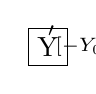
\begin{tikzpicture}[baseline]
        \Tree   [.XP
                    [.YP
                        \node [draw] {Y};
                        [.ZP \edge[roof]; {\hphantom{1em}} ]
                    ]
                    [.X$'$
                        X$_{[-\text{Y}_0-]}$
                        [.UP \edge[roof]; {\hphantom{1em}} ]
                    ]
                ]
        \end{tikzpicture}
\end{xlist}
\end{exe}
\end{minipage}
\begin{minipage}[t]{.5\textwidth}
\begin{exe}
\exi{}
    \begin{xlist}
    \exi{b.} Remove(X$'_{[-\text{Y}_0-]}$,Y):\\
        \Tree   [.XP
                    [.ZP \edge[roof]; {\hphantom{1em}} ]
                    [.X$'$
                        X
                        [.UP \edge[roof]; {\hphantom{1em}} ]
                    ]
                ]
\end{xlist}
\end{exe}
\end{minipage}
%
%
%
%\ea \emph{Remove and heads: specifiers w/o specifiers}
%
%\noindent \begin{minipage}{9cm}
%
%\ex. {\it \label{16ab}Remove and heads: specifiers w/o specifiers} \a.
%Merge(X$'$$_{[\bullet \rm Y\bullet]\succ[-Y_0-]}$,YP):\\
%\begin{tabular}{cccccccccccc} & & &\node{0}{XP}\\[4mm] &\node{1}{YP} &&& &
%\node{2}{X$'$}\\[4mm] \node{7}{\fbox{Y}}  && \node{8}{ZP} &&
%\node{10}{X$_{[\rm -Y_0-]}$} && \node{11}{UP}\\[4mm]
%&&\node{9}{~~~~~}&&&&\node{12}{~~~~~}\\ \end{tabular} \nodeconnect{0}{1}
%\nodeconnect{0}{2} \nodeconnect{1}{7} \nodeconnect{1}{8} \nodetriangle{8}{9}
%\nodeconnect{2}{10} \nodeconnect{2}{11} \nodetriangle{11}{12}
%
%\end{minipage}\hspace{1.cm}\begin{minipage}{5cm} \vspace{.6cm}
%
%\ex.[b.] Remove(X$'$$_{\rm [-Y_0-]}$,Y):\\ \begin{tabular}{cccccccccccc} &
%\node{0}{XP}\\[4mm] \node{1}{ZP} && \node{2}{X$'$}\\[4mm] \node{1a}{~~~~~}&
%\node{3}{X} && \node{4}{UP}\\[4mm] &&  & \node{11}{~~~~~}\\ \end{tabular}
%\nodeconnect{0}{1} \nodeconnect{0}{2} \nodeconnect{2}{3} \nodeconnect{2}{4}
%\nodetriangle{1}{1a} \nodetriangle{4}{11}
%
%\end{minipage} \vspace{2mm}

\noindent Next consider the situation where a complement projection YP is
removed via [$-\text{Y}_0-$] on X, but where the difference to (\ref{6cd}) is
that Y takes both a complement (WP) and a specifier (ZP).  Again, the null
hypothesis is that after YP shell removal,  WP and ZP reassemble in their
original hierarchical and linear order in the XP domain, so that structural
changes induced by the operation are minimized -- recall that a basic property
underlying Remove operations is that they change embedded structures as little
as possible. (\ref{16cd}) shows how a Remove operation triggered by X and
targeting the head of X's complement Y reassociates Y's specifier (ZP) and
complement (WP) with the projection of X: ZP becomes a new specifier of X, and
WP replaces the original YP in the complement
position.\footnote{\label{spr7s}Two remarks.  First, it is clear that the
    earlier c-command relation of X and ZP {\it is} reversed by reassociation
    of ZP as X's specifier. Still, this qualifies as the best option since the
    alternative -- reintegrating ZP as a specifier of WP -- would (a) change a
    c-command relation into a dominance relation, and (b) carry out changes in
    a domain that should not be accessible, given the Strict Cycle Condition.
    Second, the question arises of what happens if X independently has a
    feature triggering \isi{Merge} of a specifier. There are two possibilities:
    Either this specifier is already in place, or it is merged later. The
    second case is straightforward; the specifier will be merged on top of the
    existing structure. As for the first case, ZP will have to be
    reassociated below the inherent specifier of X, so as to maximize structure
preservation. Thus, the outcome is identical.}

\begin{exe}
\ex\label{16cd} Remove and heads: complements with specifiers
\end{exe}
\noindent\begin{minipage}[t]{.5\textwidth}
\begin{exe}
\exi{}
\begin{xlist}
    \exi{a.} Merge(X$_{[\bullet \text{Y}\bullet]\succ[-\text{Y}_0-]}$,YP):\\
        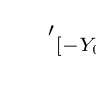
\begin{tikzpicture}[baseline]
        \Tree   [.X$'$
                    X$_{[-\text{Y}_0-]}$
                    [.YP
                        [.ZP \edge[roof]; {\hphantom{1em}} ]
                        [.Y$'$
                            \node [draw] {Y};
                            [.WP \edge[roof]; {\hphantom{1em}} ]
                        ]
                    ]
                ]
        \end{tikzpicture}
\end{xlist}
\end{exe}
\end{minipage}
\begin{minipage}[t]{.5\textwidth}
\begin{exe}
\exi{}
    \begin{xlist}
    \exi{b.} Remove(X$_{[-\text{Y}_0-]}$,Y):\\
        \Tree   [.XP
                    [.ZP \edge[roof]; {\hphantom{1em}} ]
                    [.X$'$
                        X
                        [.WP \edge[roof]; {\hphantom{1em}} ]
                    ]
                ]
\end{xlist}
\end{exe}
\end{minipage}
%\noindent \begin{minipage}{10cm}
%
%\ex. {\it \label{16cd}Remove and heads: complements with specifiers} \a.
%Merge(X$_{[\bullet \rm Y\bullet]\succ[-Y_0-]}$,YP):\\
%\begin{tabular}{cccccccccccc} & \node{0}{X$'$}\\[4mm] \node{1}{X$_{[\rm
%-Y_0-]}$} & & \node{2}{YP}\\[4mm] & \node{7}{ZP} && \node{8}{Y$'$}\\[4mm]
%&\node{7a}{~~~~~}&\node{9}{\fbox{Y}} && \node{10}{WP}\\[4mm]
%&&&&\node{11}{~~~~~} \end{tabular} \nodeconnect{0}{1} \nodeconnect{0}{2}
%\nodeconnect{2}{7} \nodeconnect{2}{8} \nodeconnect{8}{9} \nodeconnect{8}{10}
%\nodetriangle{7}{7a} \nodetriangle{10}{11}
%
%\end{minipage}\hspace{.7cm}\begin{minipage}{7cm} \vspace{-.4cm}
%
%\ex.[b.] Remove(X$_{\rm [-Y_0-]}$,Y):\\ \begin{tabular}{cccccccccccc} &
%\node{0}{XP}\\[4mm] \node{1}{ZP} & & \node{2}{X$'$}\\[4mm] \node{3}{~~~~~}&
%\node{4}{X} && \node{5}{WP}\\[4mm] &&&\node{6}{~~~~~}\\ \end{tabular}
%\nodeconnect{0}{1} \nodeconnect{0}{2} \nodeconnect{2}{4} \nodeconnect{2}{5}
%\nodetriangle{1}{3} \nodetriangle{5}{6}
%
%\end{minipage}

\noindent The derivation in (\ref{16cd}) illustrates a non-trivial property of
Remove operations applying to heads that take a complement and a specifier: ZP
undergoes  dislocation {\it without movement} (i.e., without internal \isi{Merge} of
ZP in (\ref{16cd}b)). This will play a role below.

Finally, for the sake of completeness, the scenario where the head (Y) of a
specifier (YP) is removed that takes both a complement (WP) and a specifier
(ZP) is illustrated in (\ref{6ab}).  As before, ZP and WP are reassociated with
X's projection in a way that maximally maintains earlier c-command and
linearization relations, and here this implies that ZP and WP become outer and
inner specifiers of X, respectively.

%\noindent \begin{minipage}{9cm}
%
%\ex. {\it \label{6ab}Remove and heads: specifiers with specifiers} \a.
%Merge(X$'$$_{[\bullet \rm Y\bullet]\succ[-Y_0-]}$,YP):\\
%\begin{tabular}{cccccccccccc} & & &\node{0}{XP}\\[4mm] &\node{1}{YP} &&& &
%\node{2}{X$'$}\\[4mm] \node{3}{ZP} && \node{4}{Y$'$} && \node{10}{X$_{[\rm
%-Y_0-]}$} && \node{11}{UP}\\[4mm] \node{5}{~~~~~}&\node{7}{\fbox{Y}} &&
%\node{8}{WP}&&&\node{12}{~~~~~}\\[4mm] &&&\node{9}{~~~~~}\\[4mm] \end{tabular}
%\nodeconnect{0}{1} \nodeconnect{0}{2} \nodeconnect{1}{3} \nodeconnect{1}{4}
%\nodetriangle{3}{5}\nodetriangle{8}{9} \nodeconnect{4}{7} \nodeconnect{4}{8}
%\nodeconnect{2}{10} \nodeconnect{2}{11}\nodetriangle{11}{12}
%
%\end{minipage}\hspace{1.cm}\begin{minipage}{7cm} \vspace{.2cm}
%
%\ex.[b.] Remove(X$'$$_{\rm [-Y_0-]}$,Y):\\ \begin{tabular}{cccccccccccc} &
%\node{0}{XP}\\[4mm] \node{1}{ZP} && \node{2}{X$'$}\\[4mm] \node{1a}{~~~~~}&
%\node{3}{WP} && \node{4}{X$'$}\\[4mm] &\node{3a}{~~~~~}& \node{5}{X} &&
%\node{11}{UP}\\[4mm] &&&&\node{11a}{~~~~~}\\ \end{tabular} \nodeconnect{0}{1}
%\nodeconnect{0}{2} \nodeconnect{2}{3} \nodeconnect{2}{4} \nodeconnect{4}{5}
%\nodeconnect{4}{11} \nodetriangle{1}{1a} \nodetriangle{3}{3a}
%\nodetriangle{11}{11a}
%
%\end{minipage}

\begin{exe}
\ex\label{6ab} Remove and heads: specifiers with specifiers
\end{exe}
\noindent\begin{minipage}[t]{.5\textwidth}
\begin{exe}
\exi{}
\begin{xlist}
    \exi{a.} Merge(X$'_{[\bullet \text{Y}\bullet]\succ[-\text{Y}_0-]}$,YP):\\
        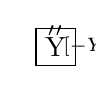
\begin{tikzpicture}[baseline]
        \Tree   [.XP
                    [.YP
                        [.ZP \edge[roof]; {\hphantom{1em}} ]
                        [.Y$'$
                            \node [draw] {Y};
                            [.WP \edge[roof]; {\hphantom{1em}} ]
                        ]
                    ]
                    [.X$'$
                        X$_{[-\text{Y}_0-]}$
                        [.UP \edge[roof]; {\hphantom{1em}} ]
                    ]
                ]
        \end{tikzpicture}
\end{xlist}
\end{exe}
\end{minipage}
\begin{minipage}[t]{.5\textwidth}
\begin{exe}
\exi{}
    \begin{xlist}
    \exi{b.} Remove(X$'_{[-\text{Y}_0-]}$,Y):\\
        \Tree   [.XP
                    [.ZP \edge[roof]; {\hphantom{1em}} ]
                    [.X$'$
                        [.WP \edge[roof]; {\hphantom{1em}} ]
                        [.X$'$
                            X
                            [.UP \edge[roof]; {\hphantom{1em}} ]
                        ]
                    ]
                ]
\end{xlist}
\end{exe}
\end{minipage}

\noindent Overall, what emerges is a principled approach to \isi{reanalysis} by
structure removal, which is also restrictive, due to the Strict Cycle
Condition. The patterns in \eqref{6cd}--\eqref{6ab} can all be shown to
underlie syntactic constructions exhibiting evidence for conflicting structure
assignments that are unrelated to restructuring infinitives. For instance,
removal of specifier heads with complements and specifiers, as in \eqref{6ab}, is
argued in \cite{Mueller:17:pre} to account for conflicting structure
assignments to  complex prefield constructions in \ili{German} (viz., as topicalized
headless VPs  and as multiple specifiers of C); removal of complement and
specifier heads with complements but no specifiers, as in \eqref{6cd} and
\eqref{16ab}, is argued in \cite{Mueller:15:str} and \cite{Puskar:16} to account
for conflicting evidence for nominals as DPs or NPs in \ili{Circassian} and
\ili{Serbo-Croatian}, respectively, and in \cite{Korsah&Murphy:17:aga} to account for
the presence or absence of clausal determiners in Kwa; and removal of
complement heads with specifiers, as in \eqref{16cd}, is argued in
\cite{Schwarzer:16} to account for conflicting evidence concerning the size of
{\it tough}-movement constructions in \ili{English} and \ili{German}. (In addition,
\citealt{Dschaak:17} develops an account of restructuring in \ili{Russian} along the
lines of the present proposal.) In the next section, I develop an approach to
restructuring that accounts for the conflicting evidence laid out in Section 2.
I will argue that the evidence for biclausality involves environments before
removal of  heads, and the evidence for monoclausality involves environments
after removal. Removal typically takes place with complements (as in
\eqref{6cd} and \eqref{16cd}), but in the context of discussing the third
construction, I will also argue that it can involve specifiers (as in
\eqref{16ab} and \eqref{6ab}).

\section{Analysis}\label{sec:32.4}

\subsection{Structure removal in infinitival complements}

Suppose that all \isi{control} verbs take CP complements.  The special property of
restructuring \isi{control} verbs then is that they can subsequently remove CP and TP
layers, yielding derived vP complements.\footnote{In principle, it is possible
    to introduce yet more subtle distinctions, with different degrees of
    removal eventually yielding different final output structures for the
    infinitival complements; see \cite{Fanselow:91},
    \cite{Wurmbrand:01,Wurmbrand:15}. Also cf.\ the remark on long-distance
passivization in footnote \ref{ldpfn} below.} More specifically, I suggest that
evidence for biclausality involves a CP structure before removal. Thus, the
relevant operations that are indicative of biclausality are counter-bled and
counter-fed by Remove. In contrast, evidence for monoclausality involves a vP
structure after removal. Consequently, the relevant operations that are
indicative of monoclausality are bled and fed by Remove.  The derivation of a
restructuring \isi{control} infinitive is shown in (\ref{cp:control}) and
(\ref{ex:restr}). In (\ref{cp:control}a), infinitival C is merged with a TP
containing an infinitival V, an object DP that has been assigned accusative\is{accusative case}
case by v, and a PRO subject that does not yet have case. Next, in
(\ref{cp:control}b), (cf.\ \Cref{b2}), infinitival C for \isi{control}
environments can value the infinitival subject with null case (see footnote
\ref{pro3}); I take this to be an instance of \isi{Agree}.\footnote{Here, asterisks
    indicate that a feature triggers an \isi{Agree} operation ([$*$F$*$]).  Also,
    since there is no obligatory \gls{EPP} feature for \ili{German} T, there is no reason
    to assume that PRO must undergo \isi{movement} to SpecT; it is licensed by C in
its in situ (Spec\emph{v}) position.}\newpage

\begin{exe}
\ex\label{cp:control} Control infinitives:
\begin{xlist}
    \ex \emph{Merge} (C$_{[\bullet
    \text{T}\bullet],[\text{$*$case:[null]$*$]}}$, \text{TP}):\\
    \begin{tikzpicture}[baseline]

        \Tree 	[.CP
                    C\textsubscript{[$*$case:[null]$*$]}
                    [.TP
                        [.\emph{v}P
                            PRO\textsubscript{[case:$\Box$]}
                            [.\emph{v}$'$
                                [.VP
                                    [.DP ihn ]
                                    [.V {zu küssen} ]
                                ]
                                \emph{v}
                            ]
                        ]
                        T
                    ]
                ]

    \end{tikzpicture}
    \ex \emph{Agree} (C$_{[\text{$*$case:[null]$*$]}}$,
    PRO\textsubscript{case:$\Box$}):\\
    \begin{tikzpicture}[baseline]

        \Tree 	[.CP
                    C
                    [.TP
                        [.\emph{v}P
                            PRO\textsubscript{[case:[null]]}
                            [.\emph{v}$'$
                                [.VP
                                    [.DP ihn ]
                                    [.V {zu küssen} ]
                                ]
                                \emph{v}
                            ]
                        ]
                        T
                    ]
                ]


    \end{tikzpicture}
\end{xlist}
\end{exe}
%\ex. {\it Control infinitives}: \a. {\it \isi{Merge} \rm (C$_{\rm [\bullet
%T\bullet],[*case:[null]*]}$, \rm TP}):\\ \begin{tabular}{cccccccccccccc}
%&\node{1}{CP} & \\[4mm] \node{2}{~~~~~~~~C$_{\rm [*case:[null]*]}$} &&
%\node{3}{TP} \\[4mm] & \node{4}{vP} && \node{5}{T}\\[4mm] \node{6}{PRO$_{\rm
%[case:\Box]}$} && \node{7}{v$'$}\\[4mm] & \node{8}{VP} && \node{9}{v}\\[4mm]
%\node{10}{DP} && \node{11}{V}\\[4mm] \node{10a}{ihn} &&
%\node{11a}{zu~küssen}\\[4mm] \end{tabular}
%\nodeconnect{1}{2}\nodeconnect{1}{3}\nodeconnect{3}{4}\nodeconnect{3}{5}\nodeconnect{4}{6}
%\nodeconnect{4}{7}\nodeconnect{7}{8}\nodeconnect{7}{9}\nodeconnect{8}{10}\nodeconnect{8}{11}
%\nodeconnect{10}{10a}\nodeconnect{11}{11a} \b. {\it \isi{Agree} \rm (C$_{\rm
%[*case:[null]*]}$, \rm PRO$_{\rm [case:\Box]}$)}:\\
%\begin{tabular}{cccccccccccccc} &\node{1}{CP} & \\[4mm] \node{2}{C} &&
%\node{3}{TP} \\[4mm] & \node{4}{vP} && \node{5}{T}\\[4mm] \node{6}{PRO$_{\rm
%[case:[null]]}$} && \node{7}{v$'$}\\[4mm] & \node{8}{VP} && \node{9}{v}\\[4mm]
%\node{10}{DP} && \node{11}{V}\\[4mm] \node{10a}{ihn} &&
%\node{11a}{zu~küssen}\\[4mm] \end{tabular}
%\nodeconnect{1}{2}\nodeconnect{1}{3}\nodeconnect{3}{4}\nodeconnect{3}{5}\nodeconnect{4}{6}
%\nodeconnect{4}{7}\nodeconnect{7}{8}\nodeconnect{7}{9}\nodeconnect{8}{10}\nodeconnect{8}{11}
%\nodeconnect{10}{10a}\nodeconnect{11}{11a}

If restructuring does not take place, that is all there is to say. However, if
the matrix \isi{control} predicate has the restructuring property, the derivation
proceeds as in (\ref{ex:restr}). The lexical property that characterizes a
restructuring verb in the present approach is that a [$-\text{C}_0-$] feature
and a [$-\text{T}_0-$] feature can be added at the bottom of its stack of
operation-triggering features. If this happens, the \isi{Merge} operation combining V
and CP (triggered by a [{\small $\bullet$}C{\small $\bullet$}] feature that
uniformly characterizes \isi{control} verbs) in (\ref{ex:restr}a) is followed by
recursive removal -- first of the CP shell (cf.\ (\ref{ex:restr}b)), and then
of the TP shell (cf.\  (\ref{ex:restr}c)).%\largerpage[2]

\begin{exe}
\ex\label{ex:restr} Restructuring:
\begin{xlist}
    \ex\label{repa} \emph{Merge} (V$_{[\bullet
    \text{C}\bullet]\succ[-\text{C}_0-]\succ[-\text{T}_0-]}$, CP):\\
        \begin{tikzpicture}[baseline]

            \Tree 	[.VP
                        [.CP
                            C
                            [.TP
                                [.\emph{v}P
                                    PRO\textsubscript{[case:[null]]}
                                    [.\emph{v}$'$
                                        [.VP
                                            [.DP ihn ]
                                            [.V {zu küssen} ]
                                        ]
                                        \emph{v}
                                    ]
                                ]
                                T
                            ]
                        ]
                        [.V$_{[-\text{C}_0-]\succ[-\text{T}_0-]}$ versucht ]
                    ]

        \end{tikzpicture}
    \ex \emph{Remove} (V$_{[-\text{C}_0-]\succ[-\text{T}_0-]}$, CP):\\
        \begin{tikzpicture}[baseline]

            \Tree 	[.VP
                        [.TP
                            [.\emph{v}P
                                PRO\textsubscript{[case:[null]]}
                                [.\emph{v}$'$
                                    [.VP
                                        [.DP ihn ]
                                        [.V {zu küssen} ]
                                    ]
                                    \emph{v}
                                ]
                            ]
                            T
                        ]
                        [.V$_{[-\text{T}_0-]}$ versucht ]
                    ]

        \end{tikzpicture}
    \newpage
    \ex\label{repb} \emph{Remove} (V$_{[-\text{T}_0-]}$, TP):\\
        \begin{tikzpicture}[baseline]

            \Tree 	[.VP
                        [.\emph{v}P
                            PRO\textsubscript{[case:[null]]}
                            [.\emph{v}$'$
                                [.VP
                                    [.DP ihn ]
                                    [.V {zu küssen} ]
                                ]
                                \emph{v}
                            ]
                        ]
                        [.V$_{[-\text{T}_0-]}$ versucht ]
                    ]

        \end{tikzpicture}
\end{xlist}
\end{exe}

%\newpage \ex. {\it Restructuring}: \a. {\it \label{repa}Merge} (V$_{\rm
%[\bullet C\bullet]\succ[-C_0-]\succ[-T_0-]}$, CP):\\
%\begin{tabular}{cccccccccccccccc} &&\node{-1}{VP}\\[4mm] &\node{1}{CP} &&
%\node{0}{\hspace{10mm}V$_{\rm [-C_0-]\succ[-T_0-]}$}\\[4mm] \node{2}{C} &&
%\node{3}{TP} &\node{0a}{versucht}\\[4mm] & \node{4}{vP} && \node{5}{T}\\[4mm]
%\node{6}{PRO$_{\rm [case:[null]]}$} && \node{7}{v$'$}\\[4mm] & \node{8}{VP} &&
%\node{9}{v}\\[4mm] \node{10}{DP} && \node{11}{V}\\[4mm] \node{10a}{ihn} &&
%\node{11a}{zu~küssen}\\[4mm] \end{tabular}
%\nodeconnect{1}{2}\nodeconnect{1}{3}\nodeconnect{3}{4}\nodeconnect{3}{5}\nodeconnect{4}{6}
%\nodeconnect{4}{7}\nodeconnect{7}{8}\nodeconnect{7}{9}\nodeconnect{8}{10}\nodeconnect{8}{11}
%\nodeconnect{10}{10a}\nodeconnect{11}{11a}\nodeconnect{-1}{1}\nodeconnect{-1}{0}\nodeconnect{0}{0a}
%\b. {\it Remove} (V$_{\rm [-C_0-]\succ[-T_0-]}$, CP):\\
%\begin{tabular}{cccccccccccccccc} &&&\node{-1}{VP}\\[4mm] &&\node{1}{TP} &&
%\node{0}{\hspace{10mm}V$_{\rm [-T_0-]}$}\\[4mm] & \node{4}{vP} && \node{5}{T}&
%\node{0a}{versucht}\\[4mm] \node{6}{PRO$_{\rm [case:[null]]}$} &&
%\node{7}{v$'$}\\[4mm] & \node{8}{VP} && \node{9}{v}\\[4mm] \node{10}{DP} &&
%\node{11}{V}\\[4mm] \node{10a}{ihn} && \node{11a}{zu~küssen}\\[4mm]
%\end{tabular} \nodeconnect{1}{4}\nodeconnect{1}{5}\nodeconnect{4}{6}
%\nodeconnect{4}{7}\nodeconnect{7}{8}\nodeconnect{7}{9}\nodeconnect{8}{10}\nodeconnect{8}{11}
%\nodeconnect{10}{10a}\nodeconnect{11}{11a}\nodeconnect{-1}{1}\nodeconnect{-1}{0}\nodeconnect{0}{0a}
%\b. {\it \label{repb}Remove} (V$_{\rm [-T_0-]}$, TP):\\
%\begin{tabular}{cccccccccccccccc} &&\node{-1}{VP}\\[4mm] &\node{1}{vP} &&
%\node{0}{V}\\[4mm] \node{6}{PRO$_{\rm [case:[null]]}$} && \node{7}{v$'$}&
%\node{0a}{versucht}\\[4mm] & \node{8}{VP} && \node{9}{v}\\[4mm] \node{10}{DP}
%&& \node{11}{V}\\[4mm] \node{10a}{ihn} && \node{11a}{zu~küssen}\\[4mm]
%\end{tabular} \nodeconnect{1}{6}\nodeconnect{1}{7}
%\nodeconnect{7}{8}\nodeconnect{7}{9}\nodeconnect{8}{10}\nodeconnect{8}{11}
%\nodeconnect{10}{10a}\nodeconnect{11}{11a}\nodeconnect{-1}{1}\nodeconnect{-1}{0}\nodeconnect{0}{0a}

The end result is a proper monoclausal
structure.\footnote{\label{whytp}Instantiation of the features for head
removal on restructuring  \isi{control} verbs is optional, and it turns out that
hardly any restrictions are needed to guarantee only correct outcomes. If the
order of the two features on V is reversed (V$_{[\bullet\text{C}\bullet] \succ
[-\text{T}_0-] \succ [-\text{C}_0-]}$), there can be no removal of TP (because of the Strict
Cycle Condition), and no removal of CP either (because [$-\text{C}_0-$] is not
active before [$-\text{T}_0-$] is discharged).  If the matrix verb  bears
[$-\text{T}_0-$] but not [$-\text{C}_0-$], restructuring also cannot take place
(because of the Strict Cycle Condition). Finally, if only [$-\text{C}_0-$] is
instantiated, restructuring to TP size would be expected. To avoid such an
outcome, it can be assumed that [$-\text{T}_0-$] and [$-\text{C}_0-$] are tied
because they are part of the same phase\is{phases}; also see \cite{Pesetsky:16}. (That
said, most of the evidence for monoclausality would not necessarily be
incompatible with a TP status of the complement; the crucial requirement is the
absence of CP.)}

\subsection{Deriving evidence for biclausality}

As noted above, the operations that presuppose the presence of CP are
counter-bled and counter-fed by structure removal: Removal simply comes too
late to bleed or feed operations that are indicative of the CP layer. Let me
go through the evidence one by one. First, consider {\it uniformity of
embedding} (\Cref{b1}).  Given that features for removal are
optional, the implicational generalization that all \isi{control} verbs that permit
restructuring are also compatible with non-restructuring complements is
derived without further ado. The only way to reach vP is via an initial CP:
Thus, Remove counter-bleeds feature-driven external \isi{Merge}.

Second, as for the {\it licensing and interpretation of PRO} (\Cref{b2}), PRO
is licensed via \isi{Agree} with an infinitival C that assigns null case to it. Once
null case is assigned, it cannot be taken away again. Thus, it does not matter
that the context in which PRO can be licensed (viz., a CP) is ultimately
destroyed by removal: Remove counter-bleeds PRO licensing.

Let me turn next to the {\it absence of new binding domains} after
restructuring (\Cref{b3}).  Assuming that reflexives are licensed by \isi{Agree}
operations which are blocked by a CP boundary, a reflexive will have its index
fixed once the minimal CP is reached. Subsequent structure removal can neither
lead to new binding options by adding a binding index on a reflexive if new
potential antecedents are around,\footnote{Also note that unlike \ili{English},
    \ili{German} does not allow for \isi{movement} producing new binding options; cf.
\cite{Barss:86} vs.\ \cite{Frey:93} and \cite{Buering:05}.} nor can it undo
existing binding indices on a reflexive: Remove counter-feeds new binding of
reflexives and counter-bleeds old binding of reflexives.

Fourth, concerning the evidence based on {\it unstressed pronoun
fronting}\is{fronting!of pronouns}
(\Cref{b4}), recall that  an unstressed pronoun moves to the left edge of vP,
but must be licensed in this position by C (perhaps as an instance of \isi{Agree}, as
suggested in footnote \ref{cupf}). Subsequent removal of CP and TP comes too
late to block the licensing: Remove counter-bleeds unstressed pronoun fronting.

Fifth, consider the argument based on {\it the third construction} (\Cref{b5}):
Extraposition of a restructuring infinitive is indicative of its CP status
because only CP can undergo extraposition in \ili{German}; TP, vP, and VP cannot do
so. This implies that CP extraposition takes place {\it before} structure
removal; otherwise the possibility of extraposition would not be explained. For
the sake of concreteness, suppose that rightward \isi{movement} is triggered by an
optional designated feature, say [$\circ$X$\circ$] (with X $\in$ $\{$C, P,
D$\}$ in \ili{German}). A relevant part of the derivation of a sentence like
\eqref{22a} is shown in (\ref{thirdder}). First, the infinitival CP is merged
to the left of V (see (\ref{thirdder}a)); then it undergoes extraposition,
which I assume to target a right-peripheral specifier position (see
(\ref{thirdder}b); but note that assuming extraposition to involve
right-\isi{adjunction} would not substantially change things). In the next two steps,
the CP and TP shells are successively removed (see
(\ref{thirdder}c,d)).\newpage

\begin{exe}
\ex\label{thirdder} The third construction:
\begin{xlist}
    \ex \emph{Merge}
    (V$_{[\bullet\text{C}\bullet]\succ[\circ\text{C}\circ]\succ[-\text{C}_0-]\succ[-\text{T}_0-]}$, CP):\\
    \begin{tikzpicture}[baseline]

        \Tree 	[.VP
                    [.CP
                        C
                        [.TP
                            [.\emph{v}P
                                PRO\textsubscript{[case:[null]]}
                                [.\emph{v}$'$
                                    [.VP
                                        [.DP ihn ]
                                        [.V {zu küssen} ]
                                    ]
                                    \emph{v}
                                ]
                            ]
                            T
                        ]
                    ]
                    [.V$_{[\circ\text{C}\circ]\succ[-\text{C}_0-]\succ[-\text{T}_0-]}$ versucht ]
                ]

    \end{tikzpicture}
    \ex \emph{Extrapose} (V$_{[\circ\text{C}\circ]\succ[-\text{C}_0-]\succ[-\text{T}_0-]}$, CP):\\
    \begin{tikzpicture}[baseline]

        \Tree 	[.VP
                    [.V$'$
                        \node (source) {--};
                        [.V$_{[\circ\text{C}\circ]\succ[-\text{C}_0-]\succ[-\text{T}_0-]}$ versucht ]
                    ]
                    [.\node(cp){CP};
                        C
                        [.TP
                            [.\emph{v}P
                                PRO\textsubscript{[case:[null]]}
                                [.\emph{v}$'$
                                    [.VP
                                        [.DP ihn ]
                                        [.V {zu küssen} ]
                                    ]
                                    \emph{v}
                                ]
                            ]
                            T
                        ]
                    ]
                ]

                \draw [->] (source.south).. controls +(south east:2.5) and +(west:2.5)
                    ..(cp.west);

    \end{tikzpicture}
    \ex \emph{Remove} (V$_{[-\text{C}_0-]\succ[-\text{T}_0-]}$, CP):\\
    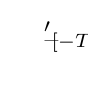
\begin{tikzpicture}[baseline]

        \Tree 	[.VP
                    [.V$'$
                        \node (source) {--};
                        [.V$_{[-\text{T}_0-]}$ versucht ]
                    ]
                    [.TP
                        [.\emph{v}P
                            PRO\textsubscript{[case:[null]]}
                            [.\emph{v}$'$
                                [.VP
                                    [.DP ihn ]
                                    [.V {zu küssen} ]
                                ]
                                \emph{v}
                            ]
                        ]
                        T
                    ]
                ]

    \end{tikzpicture}
    \ex\label{ls42} \emph{Remove} (V$_{[-\text{T}_0-]}$, TP):\\
    \begin{tikzpicture}[baseline]

        \Tree 	[.VP
                    [.V$'$
                        \node (source) {--};
                        [.V versucht ]
                    ]
                    [.\emph{v}P
                        PRO\textsubscript{[case:[null]]}
                        [.\emph{v}$'$
                            [.VP
                                [.DP ihn ]
                                [.V {zu küssen} ]
                            ]
                            \emph{v}
                        ]
                    ]
                ]

    \end{tikzpicture}

\end{xlist}
\end{exe}

%\newpage \ex. {\it The \label{thirdder}third construction}: \a. {\it Merge}
%(V$_{\rm [\bullet C\bullet]\succ[\circ C\circ]\succ[-C_0-]\succ[-T_0-]}$,
%CP):\\ \begin{tabular}{cccccccccccccccc} &&\node{-1}{VP}\\[4mm] &\node{1}{CP}
%&& \node{0}{\hspace{14mm}V$_{\rm [\circ C
%\circ]\succ[-C_0-]\succ[-T_0-]}$}\\[4mm] \node{2}{C} && \node{3}{TP}
%&\node{0a}{versucht}\\[4mm] & \node{4}{vP} && \node{5}{T}\\[4mm]
%\node{6}{PRO$_{\rm [case:[null]]}$} && \node{7}{v$'$}\\[4mm] & \node{8}{VP} &&
%\node{9}{v}\\[4mm] \node{10}{DP} && \node{11}{V}\\[4mm] \node{10a}{ihn} &&
%\node{11a}{zu~küssen}\\[4mm] \end{tabular}
%\nodeconnect{1}{2}\nodeconnect{1}{3}\nodeconnect{3}{4}\nodeconnect{3}{5}\nodeconnect{4}{6}
%\nodeconnect{4}{7}\nodeconnect{7}{8}\nodeconnect{7}{9}\nodeconnect{8}{10}\nodeconnect{8}{11}
%\nodeconnect{10}{10a}\nodeconnect{11}{11a}\nodeconnect{-1}{1}\nodeconnect{-1}{0}\nodeconnect{0}{0a}
%\b. {\it Extrapose} (V$_{\rm [\circ C\circ],[-C_0-]\succ[-T_0-]}$, CP):\\
%\begin{tabular}{cccccccccccccccc} &&\node{-1}{VP}\\[4mm]
%&\node{-2}{V$'$}&&&\node{1}{CP} && \\[4mm]
%\node{-3}{--}&&\node{0}{\hspace{1cm}V$_{\rm [-C_0-]\succ[-T_0-]}$}
%&\node{2}{C} && \node{3}{TP} \\[4mm] &&\node{0a}{versucht}&& \node{4}{vP} &&
%\node{5}{T}\\[4mm] &&& \node{6}{PRO$_{\rm [case:[null]]}$} &&
%\node{7}{v$'$}\\[4mm] &&&& \node{8}{VP} && \node{9}{v}\\[4mm] &&&\node{10}{DP}
%&& \node{11}{V}\\[4mm] &&&\node{10a}{ihn} && \node{11a}{zu~küssen}\\[4mm]
%\end{tabular}
%\nodeconnect{1}{2}\nodeconnect{1}{3}\nodeconnect{3}{4}\nodeconnect{3}{5}\nodeconnect{4}{6}
%\nodeconnect{4}{7}\nodeconnect{7}{8}\nodeconnect{7}{9}\nodeconnect{8}{10}\nodeconnect{8}{11}
%\nodeconnect{10}{10a}\nodeconnect{11}{11a}\nodeconnect{-1}{1}\nodeconnect{-1}{-2}
%\nodeconnect{-2}{-3}\nodeconnect{-2}{0}\nodeconnect{0}{0a}\anodecurve[b]{-3}[l]{1}{3cm}
%\b. {\it Remove} (V$_{\rm [-C_0-]\succ[-T_0-]}$, CP):\\
%\begin{tabular}{cccccccccccccccc} &&\node{-1}{VP}\\[4mm]
%&\node{-2}{V$'$}&&&&\node{1}{TP} && \\[4mm]
%\node{-3}{--}&&\node{0}{\hspace{1cm}V$_{\rm [-T_0-]}$} && \node{4}{vP}&&
%\node{5}{T} \\[4mm] &&\node{0a}{versucht}& \node{6}{PRO$_{\rm [case:[null]]}$}
%&& \node{7}{v$'$}\\[4mm] &&&& \node{8}{VP} && \node{9}{v}\\[4mm]
%&&&\node{10}{DP} && \node{11}{V}\\[4mm] &&&\node{10a}{ihn} &&
%\node{11a}{zu~küssen}\\[4mm] \end{tabular}
%\nodeconnect{1}{4}\nodeconnect{1}{5}\nodeconnect{4}{6}
%\nodeconnect{4}{7}\nodeconnect{7}{8}\nodeconnect{7}{9}\nodeconnect{8}{10}\nodeconnect{8}{11}
%\nodeconnect{10}{10a}\nodeconnect{11}{11a}\nodeconnect{-1}{1}\nodeconnect{-1}{-2}
%\nodeconnect{-2}{-3}\nodeconnect{-2}{0}\nodeconnect{0}{0a} \newpage\b. {\it
%\label{ls42}Remove} (V$_{\rm [-T_0-]}$, TP):\\
%\begin{tabular}{cccccccccccccccc} &&\node{-1}{VP}\\[4mm]
%&\node{-2}{V$'$}&&&\node{1}{vP} && \\[4mm] \node{-3}{--}&&\node{0}{V}
%&\node{6}{PRO$_{\rm [case:[null]]}$} && \node{7}{v$'$} \\[4mm]
%&&\node{0a}{versucht}&  & \node{8}{VP} && \node{9}{v}\\[4mm] &&&\node{10}{DP}
%&& \node{11}{V}\\[4mm] &&&\node{10a}{ihn} && \node{11a}{zu~küssen}\\[4mm]
%\end{tabular}
%\nodeconnect{1}{6}\nodeconnect{1}{7}\nodeconnect{7}{8}\nodeconnect{7}{9}\nodeconnect{8}{10}\nodeconnect{8}{11}
%\nodeconnect{10}{10a}\nodeconnect{11}{11a}\nodeconnect{-1}{1}\nodeconnect{-1}{-2}
%\nodeconnect{-2}{-3}\nodeconnect{-2}{0}\nodeconnect{0}{0a}

As for the steps in (\ref{thirdder}c,d), recall that there is no problem with
Remove affecting specifiers (or adjuncts) rather than complements (cf.\
\eqref{16ab} and \eqref{6ab}). As a matter of fact, there is clear independent
evidence for the general possibility of restructuring with specifiers in
German.  Examples like (\ref{ex:end}a,b), where scrambling takes place from a
subject infinitive, are entirely unproblematic ((\ref{ex:end}b) may involve a
derived subject, but (\ref{ex:end}a) certainly does not).\newpage

\ea\label{ex:end} \ili{German}
    \ea
        \gll dass es$_1$ sich nicht [ PRO t$_1$ zu beanstanden~] {gehört hat}\\
            that it$_1$ \Refl{} not {} {} {}  to {object to} {acceptable is}\\
    \ex
        \gll dass sich$_1$ ihm [ PRO t$_1$ zu befreien~] {gelungen ist}\\
            that \Refl{} him\textsubscript{\Dat}  {} {} {} to free {successful was}\\
    \z
\z

The final representation in (\ref{thirdder}d) is monoclausal, as required for
scrambling and unstressed pronoun fronting\is{fronting!of pronouns} to a vP specifier of the matrix V.
However, there is a problem: It is not quite clear why a vP in a derived
specifier (or adjoined) position does not block extraction via the
\glsdesc{CED} (\glsunset{CED}\gls{CED};
\citealt{Huang:82,Chomsky:86,Cinque:90}).  I will address this issue in the
following section. With this proviso, we can conclude that Remove
counter-bleeds extraposition: Loss of the CP status of the complement in the
extraposed position comes too late to block rightward \isi{movement} (which requires
CP status).\footnote{The derivation in (\ref{thirdder}) also gives rise to
    another question: The third construction is possible with periphrastic verb
    forms; i.e., as an alternative to {\it versucht} \enquote*{tried}, as in
    \eqref{22a}, there is also the option of {\it versucht hat} \enquote*{tried
    has}, as in \eqref{22b}. There are (at least) two ways to account for this.
    First, one might assume that periphrasis comes about by \isi{head movement} of
    non-finite lexical V to the auxiliary\is{auxiliaries}, followed by discharge of the
    extraposition feature in the derived position; this would require a minimal
    modification of the Strict Cycle Condition that incorporates the effect of
(this type of) \isi{head movement}. Second, one might postulate that the two Vs form
a single complex head (see, e.g., \citealt{Zwart:16} for a recent version of
this approach); verb-second \isi{movement} might then proceed  by excorporation.}

\subsection{Deriving evidence for monoclausality}

%\largerpage[2]
\glsunset{LF}
The basic pattern is that operations that presuppose monoclausality are bled
and fed by Remove. Let me begin with the simplest cases. First, wide scope of
{\it negation} in restructuring contexts (\Cref{m6}) follows
straightforwardly: Scope is an \gls{LF}-related phenomenon that is determined
on the basis of output representations like \eqref{repb}, i.e., after structure
removal. Hence, at the stage where the  scope of the embedded negation is
determined, there is no intermediate clause boundary anymore that might prevent
wide scope (or, for that matter, permit embedded scope):  Remove feeds scope of
negation.\footnote{There is a qualification, though. As observed by
    \cite{Santorini&Kroch:91}, negation is always clause-bound in the third
    construction; cf.\ (i) vs.\ \eqref{negw3}.

\begin{exe}
    \exi{(i)} \ili{German}\\
    \gll dass ich seinen neusten Roman beschlossen habe [\textsubscript{vP} nicht zu lesen~]\\
        that I his newest novel\textsubscript{\Acc} decided have {} not to read\\
    \trans (only narrow scope)
\end{exe}

This suggests that, unlike displacement, wide scope is blocked by a vP in a
derived (specifier or adjunct) position.} Second, similar considerations apply
in the case of {\it intonation} (\Cref{m7}). The determination of intonational
breaks is a \gls{PF} process; consequently, it is output representations like
\eqref{repb} that are taken into account in order to decide whether
intonational breaks can or cannot occur -- and after  removal, the clause
boundary that is indicative of an intonational break is gone: Remove bleeds the
generation of smaller intonational phrases.

Next, \Cref{m1} (scrambling and unstressed pronoun fronting), \Cref{m3}
(extraposition), and \Cref{m4} (multiple \isi{sluicing}) all involve evidence for
monoclausality based on the a priori unexpected option of extraction (of
certain \isi{movement} types) to take place across a clause boundary with
restructuring. An obvious account might therefore rely on the assumption that
extraction from the infinitival complement can take place from the in situ
position after removal of CP and TP shells, i.e., that Remove directly feeds
extraction in the case of \isi{movement} types that cannot cross a CP boundary.
However, there are two problems with this simple view.  The first problem
concerns successive cyclicity: In general, a phrase that is supposed to undergo
extraction from a constituent needs to undergo intermediate \isi{movement} steps to
phase edges, because of the \gls{PIC}. Accordingly, an item within an
infinitival CP that will target a position in the matrix clause (e.g., via
scrambling or extraposition) does not know that eventually, there will be no CP
(due to removal by the matrix verb); thus, without look-ahead, it will have to
undergo \isi{movement} first to Specv, and then to SpecC.

The second problem has already been noted above: Recall that a vP in a
right-peripheral SpecV position should block scrambling in the third
construction, because of the \gls{CED} (see \eqref{ls42}). Taken together,
these two problems suggest that the way in which Remove feeds extraction
options is somewhat different from the way envisaged under the simple account
just sketched.

As a first step to a solution, let us assume that there is some constraint
against improper \isi{movement} that ensures that a CP blocks \isi{movement} to a
clause-external position in the case of scrambling and unstressed pronoun
fronting (cf.\ \eqref{lds1}, \eqref{lds1a}, \eqref{scr56}, \eqref{scr57}) and
extraposition (cf.\ \eqref{cp0}, \eqref{cp1}), but not with wh-movement,
\isi{topicalization} or relativization.\is{relative clauses}  There are various proposals in the
literature as to how the prohibition against \isi{movement} to low (vP- or
TP-internal) positions from a CP can be derived (see, e.g.,
\citealt[Ch.~2]{Mueller:14:buf}, \citealt{Wurmbrand:15}, and \citealt{Keine:16}
for three recent attempts); for present purposes, it may suffice to state that
such \isi{movement} (as an instance of Merge) is blocked.

On this basis, consider again the case of scrambling from a restructuring
infinitive, as in (\ref{9q}), repeated here as (\ref{ex:fritz}).\newpage

\ea\label{ex:fritz} \ili{German}\\
    \gll dass \label{fdsc4}den Fritz$_1$ keiner [ PRO t$_1$ zu küssen~] versuchte\\
        that the Fritz\textsubscript{\Acc} no-one\textsubscript{\Nom} {} {} {}  to kiss tried\\
\z

Before the infinitival CP is merged with the matrix V, successive-cyclic
movement of the embedded object DP {\it den Fritz} takes place to Spec\emph{v}
and SpecC; cf.\ (\ref{cp:movement}).

\begin{exe}
\ex\label{cp:movement} Movement in the embedded CP:\\
    \begin{tikzpicture}[baseline]

        \Tree 	[.CP
                    [.\node(dp){DP}; \edge[roof]; {den Fritz} ]
                    [.C$'$
                        C
                        [.TP
                            [.\emph{v}P
                                \node (int) {--};
                                [.\emph{v}$'$
                                    PRO\textsubscript{[case:[null]]}
                                    [.\emph{v}$'$
                                        [.VP
                                            \node (t) {--};
                                            [.V {zu küssen} ]
                                        ]
                                        \emph{v}
                                    ]
                                ]
                            ]
                            T
                        ]
                    ]
                ]

        \node [below=.5cm of dp] (fritz) {};
        \draw [arrow, bend left=45] (t) to (int);
        \draw [arrow, bend left=45] (int) to (fritz);

    \end{tikzpicture}
\end{exe}

%%\newpage
%\ex. {\it Movement in the embedded CP}:\\ \begin{tabular}{cccccccccccccccc}
%&\node{-1}{CP}&\\[4mm] \node{0}{DP}&&\node{1}{C$'$} && \\[8mm] \node{0a}{den
%Fritz}&\node{2}{C} && \node{3}{TP} &\\[4mm] && \node{4}{vP} &&
%\node{5}{T}\\[4mm] & \node{6}{--} && \node{7}{v$'$}\\[4mm] &&
%\node{8}{PRO$_{\rm [case:[null]]}$} && \node{9}{v$'$}\\[4mm] &&&\node{9a}{VP}
%&& \node{9b}{v}\\[4mm] &&\node{10}{--} && \node{11}{V}\\[4mm] && &&
%\node{11a}{zu~küssen}\\[4mm] \end{tabular}
%\nodeconnect{1}{2}\nodeconnect{1}{3}\nodeconnect{3}{4}\nodeconnect{3}{5}\nodeconnect{4}{6}
%\nodeconnect{4}{7}\nodeconnect{7}{8}\nodeconnect{7}{9}\nodeconnect{9a}{10}\nodeconnect{9a}{11}
%\nodetriangle{0}{0a}\nodeconnect{11}{11a}\nodeconnect{-1}{1}\nodeconnect{-1}{0}
%\nodeconnect{9}{9a}\nodeconnect{9}{9b}\anodecurve[b]{10}[b]{6}{2cm}\anodecurve[l]{6}[b]{0a}{1cm}

%\largerpage[2]
Next, V combines with CP (see (\ref{second}a)); then Remove(V,CP) takes place
(see (\ref{second}b)). Importantly, DP and TP, as the original specifier and
complement of C, are now both reassociated with the matrix V projection in a
structure-preserving way, and this means that DP ends up as a specifier of
matrix V without having undergone \isi{movement} to this position. Consequently,
there can be no violation of the constraint against improper \isi{movement} (improper
movement can only occur if there is \isi{movement} in the first place).\footnote{See,
    however, \cite{Keine:16} for evidence that long-distance
    agreement\is{agreement!long-distance agreement} is
    subject to the same kinds of restrictions as \isi{movement} and can also qualify
    as improper. On this more general view, only operations triggered by
features can count as improper; reassociation after structure removal still
cannot do so.} After this, V removes the TP shell (see (\ref{second}c)), which
has no further consequences for the moved DP.

\begin{exe}
\ex\label{second} Extraction and Restructuring:
\begin{xlist}
    \ex \emph{Structure before removal}:\\
    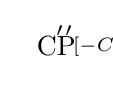
\begin{tikzpicture}[baseline]

        \Tree 	[.VP
                    [.\node(cp){CP};
                        [.DP \edge [roof]; {den Fritz} ]
                        [.C$'$
                            C
                            [.TP
                                [.\emph{v}P
                                    PRO\textsubscript{[case:[null]]}
                                    [.\emph{v}$'$
                                        [.VP {zu küssen} ]
                                        \emph{v}
                                    ]
                                ]
                                T
                            ]
                        ]
                    ]
                    [.V$_{[-\text{C}_0-]\succ[-\text{T}_0-]}$ versuchte ]
                ]

    \end{tikzpicture}
    \ex \emph{Remove} (V$_{[-\text{C}_0-]\succ[-\text{T}_0-]}$, CP),
        reassociation of DP:\\
    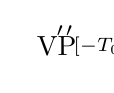
\begin{tikzpicture}[baseline]

        \Tree   [.\node(cp){VP};
                    [.DP \edge [roof]; {den Fritz} ]
                    [.V$'$
                        [.TP
                            [.\emph{v}P
                                PRO\textsubscript{[case:[null]]}
                                [.\emph{v}$'$
                                    [.VP {zu küssen} ]
                                    \emph{v}
                                ]
                            ]
                            T
                        ]
                        [.V$_{[-\text{T}_0-]}$ versuchte ]
                    ]
                ]

        \end{tikzpicture}
    \newpage
    \ex \emph{Remove} (V$_{[-\text{T}_0-]}$, TP):\\
        \begin{tikzpicture}[baseline]

        \Tree 	[.VP
                    [.DP \edge [roof]; {den Fritz} ]
                    [.V$'$
                        [.\emph{v}P
                            PRO\textsubscript{[case:[null]]}
                            [.\emph{v}$'$
                                [.VP {zu küssen} ]
                                \emph{v}
                            ]
                        ]
                        [.V versuchte ]
                    ]
                ]

        \end{tikzpicture}
\end{xlist}
\end{exe}

%\ex. {\it \label{second}Extraction and Restructuring}: \a. {\it Structure
%before removal}:\\ \begin{tabular}{cccccccccccccccc} &&\node{-2}{VP}\\[4mm]
%&\node{-1}{CP} && \node{-3}{\hspace{10mm}V$_{\rm [-C_0-]\succ[-T_0-]}$}\\[4mm]
%\node{0}{DP}&&\node{1}{C$'$} &\node{-3a}{versuchte}& \\[8mm] \node{0a}{den
%Fritz}&\node{2}{C} && \node{3}{TP} &\\[4mm] && \node{4}{vP} &&
%\node{5}{T}\\[4mm] & \node{6}{PRO$_{\rm [case:[null]]}$} &&
%\node{7}{v$'$}\\[4mm] && \node{8}{VP} && \node{9}{v}\\[4mm]
%&&\node{8a}{zu~küssen} && \\[4mm] \end{tabular}
%\nodeconnect{1}{2}\nodeconnect{1}{3}\nodeconnect{3}{4}\nodeconnect{3}{5}\nodeconnect{4}{6}
%\nodeconnect{4}{7}\nodeconnect{7}{8}\nodeconnect{7}{9}\nodeconnect{8}{8a}
%\nodeconnect{-2}{-1}\nodeconnect{-2}{-3}\nodeconnect{-1}{0}\nodeconnect{-1}{1}\nodetriangle{0}{0a}\nodeconnect{-3}{-3a}
%\b. {\it Remove} (V$_{\rm [-C_0-]\succ[-T_0-]}$, CP), reassociation of DP:\\
%\begin{tabular}{cccccccccccccccc} &&\node{-1}{VP} && \\[4mm]
%&\node{0}{DP}&&\node{1}{V$'$} && \\[8mm] &\node{0a}{den Fritz}& \node{3}{TP}
%&&\node{-3}{\hspace{10mm}V$_{\rm [-T_0-]}$} \\[4mm] & \node{4}{vP} &&
%\node{5}{T}&\node{-3a}{versuchte}\\[4mm] \node{6}{PRO$_{\rm [case:[null]]}$}
%&& \node{7}{v$'$}\\[4mm] & \node{8}{VP} && \node{9}{v}\\[4mm]
%&\node{8a}{zu~küssen} && \\[4mm] \end{tabular}
%\nodeconnect{-3}{-3a}\nodeconnect{-1}{0}\nodeconnect{-1}{1}\nodeconnect{3}{4}\nodeconnect{3}{5}\nodeconnect{4}{6}
%\nodeconnect{4}{7}\nodeconnect{7}{8}\nodeconnect{7}{9}\nodeconnect{8}{8a}
%\nodeconnect{1}{3}\nodeconnect{1}{-3}\nodetriangle{0}{0a} \b. {\it Remove}
%(V$_{\rm [-T_0-]}$, TP):\\ \begin{tabular}{cccccccccccccccc} &&\node{-1}{VP}
%&& \\[4mm] &\node{0}{DP}&&\node{1}{V$'$} && \\[8mm] &\node{0a}{den Fritz}&
%\node{3}{vP} &&\node{-3}{V} \\[4mm] & \node{4}{PRO$_{\rm [case:[null]]}$} &&
%\node{5}{v$'$}&\node{-3a}{versuchte}\\[4mm] && \node{8}{VP} &&
%\node{9}{v}\\[4mm] &&\node{8a}{zu~küssen} && \\[4mm] \end{tabular}
%\nodeconnect{-3}{-3a}\nodeconnect{-1}{0}\nodeconnect{-1}{1}\nodeconnect{3}{4}\nodeconnect{3}{5}
%\nodeconnect{5}{8}\nodeconnect{5}{9}\nodeconnect{8}{8a}
%\nodeconnect{1}{3}\nodeconnect{1}{-3}\nodetriangle{0}{0a}

\largerpage
As a consequence, DP shows up in the matrix domain without having undergone
movement itself, and is now free to move on, yielding, e.g., \eqref{fdsc4}, or,
alternatively, to stay in place, with no effects that would be directly
discernible since it cannot have crossed matrix VP material (see \cref{spr7s}).

This explains why scrambling and unstressed pronoun fronting\is{fronting!of pronouns} can take place
from restructuring infinitives.\footnote{It should be noted that the present
    analysis does not per se exclude cases like (i-b), where successive-cyclic
    long-distance \isi{movement} takes place from a position in CP$_3$ to the
    specifier of CP$_2$ (cf.\ (i-a)), followed by structure removal induced by
    the restructuring predicate {\it versuchen} \enquote*{try}, subsequent
    reassociation of DP$_0$ (plus further scrambling) in the matrix domain, and
    finally extraposition of CP$_3$.

\begin{exe}
\exi{(i)}
\begin{xlist}
    \ex[]{
    \gll[\textsubscript{VP} [\textsubscript{CP$_2$} dieses Buch$_0$
    [\textsubscript{C$'$} C [\textsubscript{TP} [\textsubscript{\emph{v}P} t$_0''$ PRO [\textsubscript{VP} [\textsubscript{CP$_3$}
    t$'_0$ [\textsubscript{C} dass~] man t$_0$ lesen soll~] [\textsubscript{V}
    vorzuschlagen~]] \emph{v}~] T~]]] [\textsubscript{V}
versucht hat~]]\\
            {} {} this book\textsubscript{\Acc} {} {} {} {} {} {} {} {} {} {} that
        one\textsubscript{\Nom} {} read should {} {to suggest} {} {} {} tried has\\}
    \ex[?*]{
        \gll dass dieses Buch$_0$ keiner [\textsubscript{VP}
        [\textsubscript{\emph{v}P} t$''_0$ PRO [\textsubscript{VP} t$_3$
        [\textsubscript{V} vorzuschlagen~]] \emph{v}~]
        [\textsubscript{V} versucht hat~]] [\textsubscript{CP$_3$} t$'_0$
        [\textsubscript{C} dass~] man t$_0$ lesen soll~]\\
        that this
book\textsubscript{\Acc} no-one\textsubscript{\Nom} {} {}  {} {} {} {} {} {to suggest} {} {} tried has
{} {} {} that one\textsubscript{\Nom} {} read should  \\}
\end{xlist}
\end{exe}

In contrast, if the fronted object {\it dieses Buch} undergoes
\isi{topicalization}
in the same context, there is a marked improvement (but no full
acceptability). For the time being, I will leave open the question of whether
the ill-formedness of (i-b) can (or should) be made to follow from a general
constraint against improper \isi{movement}, or should be taken to indicate a
cumulative effect resulting from the choice of several marked options in the
syntax of \ili{German} (among them extraction from {\it dass} clauses and complexity
of matrix predicate ({\it vorzuschlagen versucht hat})).}

The reasoning is basically identical with extraposition: The improper \isi{movement}
effect in the presence of a CP (see \eqref{cp01}) can be circumvented after CP
removal in restructuring contexts (see \eqref{cp20}).

As for recoverability-driven fronting\is{fronting!of wh-phrases} of wh-phrases in multiple \isi{sluicing}
contexts (cf.\ \eqref{2unbe1} vs.\ \eqref{unlod28}, \eqref{2unbe}), recall that
there are three competing approaches: The second wh-phrase may have undergone
scrambling \parencite{Sauerland:99:loc}, extraposition
\parencite{Lasnik:14:mul}, or wh-movement \parencite{Heck&Mueller:03:vers}.
Assuming that the relevant distinctions in the latter type of approach are due
to an {\it initial} presence or absence of a CP projection, such that the
second wh-movement in the embedded domain is blocked in the presence of a CP
(as argued in \citealt{Heck&Mueller:03:vers}), we now have a theory-internal
argument for the former two approaches (which are both compatible with an
initial presence of CP that is subsequently undone by removal).

The final movement-related issue to be addressed concerns scrambling in the
third construction; cf.\ the examples in \eqref{third} and the derivation in
\eqref{thirdder}. Recall that the problem with the derivation resulting in
\eqref{ls42} is that scrambling from the vP in the extraposed position
should violate the \gls{CED}.  This problem is now solved: Almost exactly the
same derivation as in \eqref{second} takes place with extraction in the third
construction, the only difference being that CP is extraposed prior to removal.
Thus, a DP that is in SpecC of the extraposed CP becomes reassociated with VP
as a consequence of CP removal in the extraposed position. As before, this
means that a DP that has reached SpecC of a restructuring infinitive ends up in
the matrix VP domain without having undergone \isi{movement} to that position; and as
before, two possibilities arise:  First, DP can undergo further \isi{movement} in the
matrix clause (including scrambling and unstressed pronoun \isi{movement}). Second,
DP may stay in SpecV; since it has not moved there, the position is virtually
indistinguishable from a base-merged position at this point. I would like to
contend that this second option does indeed have discernible empirical effects:
It  provides a principled approach to {\it pseudo-scrambling} phenomena as they
have been identified by \cite{Geilfuss:91}.

The relevant observation is that items in immediately preverbal positions in
the third construction do not exhibit the characteristic properties of {\it
scrambling} in \ili{German}; they instantiate what has been called  {\it
pseudo-scrambling}.  \cite{Geilfuss:91} presents evidence  from a variety of
different phenomena, among them focus projection, wh-scrambling, scope,
non-specific indefinites, directional PPs, extraction, idioms, and quantifier
floating. Let me just briefly address two of them. First, (\ref{ex:marchen}a) shows that
maximal focus projection in out-of-the-blue contexts is normally impossible
with scrambled items; in contrast, (\ref{ex:marchen}b) shows that a pseudo-scrambled DP
in the third construction permits focus projection (the effect goes away again
if DP$_1$ were to undergo further displacement to a position in front of the
matrix object). In the present approach, this is accounted for
straightforwardly: focus projection is incompatible with scrambling, and the
pseudo-scrambled DP in (\ref{ex:marchen}b) is not moved but transported to
matrix SpecV via reassociation after CP removal.

\ea\label{ex:marchen} \ili{German}
    \ea[\#]{
    \gll Fritz hat das {\sc Mär}chen$_1$ einem Kind t$_1$ vorgelesen\\
        Fritz\textsubscript{\Nom} has the {fairy tale}\textsubscript{\Acc} a child\textsubscript{\Dat} {} {read to}\\}
    \ex[]{
    \gll Fritz hat einem Kind das {\sc Mär}chen$_1$ [\textsubscript{VP} versucht [ t$_1$ vorzulesen~]]\\
        Fritz\textsubscript{\Nom} has a child\textsubscript{\Dat} the {fairy tale}\textsubscript{\Acc} {} tried {} {} {to read to}\\}
    \z
\z

Second, relative scope illustrates the same effect. Normally, scrambling of one
quantified DP across another one leads to scope ambiguities (see
(\ref{ex:geschenk}a)). However, extremely local pseudo-scrambling from third
construction environments does not (see (\ref{ex:geschenk}b)). Given the
present analysis, DP$_1$ in (\ref{ex:geschenk}b) does not exhibit this property
indicative of \isi{movement} for the simple reason that it has reached its position
not by \isi{movement}, but by reassociation after CP removal.

\ea\label{ex:geschenk} \ili{German}
    \ea
    \gll Er hat mindestens ein Geschenk$_1$ fast jedem Gast t$_1$ überreicht\\
        he\textsubscript{\Nom} has {at least} one present\textsubscript{\Acc} almost every guest\textsubscript{\Dat} {} given\\
    \trans {\it Readings}: $\exists$ $>$ $\forall$, $\forall$ $>$ $\exists$
    \ex
    \gll Er hat mindestens ein Geschenk$_1$ versucht [ fast jedem Gast t$_1$ zu überreichen~]\\
        he\textsubscript{\Nom} has {at least} one present\textsubscript{\Acc} tried {} almost every guest {} to give\\
    \trans {\it Readings}: $\exists$ $>$ $\forall$, *$\forall$ $>$ $\exists$
    \z
\z

To sum up, assuming that the {\it  compactness} property (\Cref{m5}), to the
extent that it holds, can be accounted for in one of the ways suggested in the
literature, the empirical evidence for monoclausality highlighted in
\Cref{sec:32.2.1} has been derived in toto.

More generally, I would like to conclude that a Remove-based approach to
restructuring infinitives embedded under \isi{control} verbs in \ili{German} is
conceptually viable and empirically motivated; in fact, an analysis in terms
of structure removal would seem to be the only kind of principled approach
that captures both the evidence for biclausality and the evidence for
monoclausality in a straightforward way. Furthermore, the option of deriving
local displacement in restructuring contexts as a consequence of reassociation
after removal (rather than by \isi{movement}) offers a new look on pseudo-scrambling
in the third construction (and possibly in other contexts as well). All in
all, then, it seems to me that there is every reason to return to classical
concepts of restructuring as involving a genuine syntactic reduction of clause
size; the core problem with these approaches -- viz., that the analyses were
not sufficiently principled and restricted -- can be solved when an elementary
operation Remove is identified as the complete mirror image of
Merge.\footnote{\label{ldpfn}Needless to say, there are many more aspects of
restructuring  that will ultimately have to be addressed, both in \ili{German} and,
particularly, when it comes to extending the analysis to other languages. Let
me just mention two issues that I cannot address here for lack of space.
First, {\it long-distance passivization} has played an important role in the
development of restructuring theories  (see \citealt{Hoehle:78},
\citealt{Wurmbrand:01,Wurmbrand:15:com,Wurmbrand:15}, \citealt{Sternefeld:06},
\citealt{Haider:10}, and \citealt{Keine&Bhatt:16}, among many others). In
\cite{Mueller:17:ldp}, I sketch an analysis in terms of Remove that extends
the present analysis.

Second, I have been silent  about {\it status government} (see
\citealt{Bech:55,Fabb:84}), which is also sometimes viewed as being indicative
of restructuring. See \cite{Benz:19} on how the concept of status government
interacts with a Remove-based approach to restructuring.}

\printchapterglossary{}

\section*{Acknowledgments}

This paper is dedicated to Ian Roberts.  For comments and discussion, I am
grateful to  Johanna Benz, Benjamin Bruening, Christina Dschaak, Johannes
Eng\-lisch, Gisbert Fanselow, Silke Fischer, Kleanthes Grohmann, Fabian Heck,
Daniel Hole, Dalina Kallulli, Sampson Korsah,  Lanko Maru\v{s}i\v{c}, Andrew
Murphy,  Andrew Nevins, David Pesetsky, Marie-Luise Schwarzer, Volker
Struckmeier,  L\'ida Veselovsk\'a,   Philipp Weisser, Susi Wurmbrand, two
anonymous reviewers, and audiences at Universit{\"a}t Leipzig (Workshop on
Shrinking Trees), Leucorea Wittenberg (Workshop on Genus Verbi),
Universit{\"a}t Stuttgart, Universität Wien (Workshop on Passives), Tel Aviv
University (IATL 33), and SinFonIJA X in Dubrovnik.  Research for this article
was supported by a DFG Reinhart Koselleck grant (MU 1444/14-1, {\it Structure
Removal in Syntax}).

{\sloppy
\printbibliography[heading=subbibliography,notkeyword=this]
}

\end{document}
